% This file should be replaced with your file with an thesis content.
%=========================================================================
% Authors: Michal Bidlo, Bohuslav Křena, Jaroslav Dytrych, Petr Veigend and Adam Herout 2019

% For compilation piecewise (see projekt.tex), it is necessary to uncomment it and change
% \documentclass[../projekt.tex]{subfiles}
% \begin{document}

\chapter{Introduction}
% Finite Automata + Mata

Finite automata can be found in numerous fields both in research and in practice.
There are several automata libraries, each with their own set of supported automata types and operations.
Their respective design decisions gives various advantages and disadvantages for each library.
Recently, a new finite automata library, called \mata, emerged.
\mata aims to remain simple, yet perform very fast for a large set of automata operations commonly used in various applications such as string constraints solving, reasoning about regular expressions, regular model checking, or in decision procedures for logics such as WS1S or quantified Presburger arithmetic.

Efficiency of automata algorithms used in these fields is crutial since problems from all of these fields are computationally hard.
Many automata libraries are well-optimized on only one subset of operations, or presume a certain general approach to using them.
\mata points at fast computation of operations in various frameworks, providing optimized general operations on finite automata as well as several purpose-specific algorithms used in specific fields.

\mata's underlying data structures are designed in such a way that they provide sufficient performance, but also enable easy modification by the user for their own uses and extensible framework for adding new automata types, purpose-specific operations, or additional maintanence of related context while keeping the existing infrastructure working with as minimal number of changes required as possible.

In this work, we intend on utilizing the extensibility of \mata and its underlying data structures to add support for finite state transducers while maintaining the main ideas of \mata: being fast, and easy to extend or modify.

% Finite Transducers
Finite transducers are finite-state machines.
They are similar to finite automata, but finite transducers work with multiple memory tapes.
Each tape represents a regular language where finite transducers performs mapping between these languages, and, more preciselly, between words in each language.
Finite transducers model relations (called \emph{rational relations}) between regular languages, subsets of carthesian product of regular languages.
Heneforth, each finite transducer can be thought of as a translator translating (transducing) between the languages (a 2-tape finite transducer precisely models a translator from an input language to a output language, modelling a so-called \emph{binary rational relation}), a subset of $\Sigma^* \times \Sigma^*$.
In this work, we usually work with binary rational relations, but in general an \emph{n-ary rational relation} can be modelled by a n-tape transducer.

% String Solving + Noodler
In the recent decades, we have seen a rapid growth of  various procedures for SMT string solving, implemented in numerous state-of-the-art SMT solvers.
The importance of efficient algorithms for deciding satisfiability of SMT formulae is underlined by everyday applications in the industry such as AWS~\cite{Rungta2022} or the ongoing anual competion SMT-COMP~\cite{smt_comp}.

Recent advances in analysis of programs manipulating strings, string solving, automatically solving string constraints over string languages, have heightened the importance of modelling string replacement operations.
Such operations allow for replacing a substring specified by a regular language with another string.
The appliations are widely used in web applications such as implicit browser transductions, or replace functions such as \emph{replace} and \emph{replace-all} functions.
One of the most important applications of string-replace operations is defense against attacks such as cross-site scripting or code injection in web applications.
Untrusted inputs from a user are to be sanitized (e.g. by escaping the input string) in order to prevent arbitrary malicious code execution.
We need a toolset to verify that such sanitizations are correct and safe.
SMT solver with support for replace operations can be used to decide this.

Another applications are implicit browser transductions.
HTML codes need to be coded and decoded in the input strings (replacing \texttt{\&\#39;} by a single quote \texttt{'}).
% Application of transducers for string solving
Finite transducers are ideal for modelling both the sanitization operations as well as the implicit browser transductions:
Both these applications create relations between two languages, mapping strings from one language to the other which can be modelled by finite transducers.
Finite transducers can model implicit browser transductions directly.
They can be used to model string-replace operations for sanitization operations and the resulting replacement (the generated language) can be tested for emptiness of intersection with the typical cross-site scripting attack patterns database, represented as a regular languages.
Such constraints are presented to an SMT solver to decide its satisfiability.

We have previously introduced a new SMT string solver \noodler which utilizes an automata-based approach to string solving with finite automata and operations on them implemented in \mata as the backbone of the whole decision procedure of \noodler.

\paragraph{Contribution.}
In this work, we study automata models called finite transducers and their applicability to string solving. We implement the proposed solution in \mata and evaluate the implemented solution on variety of benchmark problems from practice.

Namely, the constributions of this work can be summarized as follows:
\begin{itemize}
  \item Design of data structures and algorithms for finite transducers with regard to existing and planned data structures and algorithms in \mata.
  \item Implementation of the proposed data structures and algorithms in automata library \mata,
  \item A new benchmark of replace operations encoded as finite transducers derived from SMT-LIB benchmarks with replace operations. The operations in the benchmark performed are the typically used operations in string solving on real problems, and
  \item Experimental evaluation of the implemented algorithms on a variety of benchmark problems from practice.
\end{itemize}

\chapter{Preliminaries}
\label{sec:Preliminaries}
In this chapter, we will define several terms and notions used throughout this thesis.
We follow the usual definitions of automata theory, as used in works such as~\cite{Esparza} or~\cite{Sipser} with custom modifications and additions.

\paragraph{Alphabets.}
We define an \emph{alphabet} $\Sigma = \{ a, b, c, \ldots \}$ as a set of \emph{symbols} where
symbols are usually denoted by $a, b, c, \ldots$.
$\Sigma^*$ denotes a set of all finite \emph{words} (or \emph{strings}) over the alphabet $\Sigma$.
We usually denote words $u, v, w, \ldots$.
$u[n:m]$ represents a substring of $u$ containing symbols in the interval of indices (indexed from 0) between $n$ and $m$ (including the symbol on the index $n$ and excluding the symbol on index $m$).
Furthermore, we use two special symbols: an \emph{epsilon symbol} $\eps \notin \Sigma$, representing an empty symbol (or word, $\eps \in \Sigma^*$), and a \emph{don't care symbol}, denoted $\dontCare$, representing any single symbol from $\Sigma$.
\emph{Alphabet with epsilon symbols} (epsilons) is denoted $\SigmaEps = \Sigma \cup \{ \eps \}$.

We denote \emph{concatenation} on words $w_1$, $w_2$ using $w_1 \concat w_2$, sometimes for convenience omitting the concatention operator $w_1w_2$, where $\eps$ is the neutral element of concatenation ($\eps \concat w_1 = w_1 \concat \eps = w_1$).

\section{Finite Automata}

In this section, we lay foundation to finite automata and their aspects which are utilized in this work.

\paragraph{Nondeterministic finite automata.}
A \emph{nondeterministic finite automaton} (\emph{NFA}) over the alphabet $\Sigma$ is a 5-tuple $\aut = (\states, \Sigma, \post, \initialStates, \finalStates)$ where
\begin{itemize}
    \item $\states$ is a finite set of \emph{states},
    \item $\Sigma$ is the alphabet of $\aut$,
    \item $\post: \states \times \Sigma \rightarrow 2^{\states}$ is a \emph{symbol-post function} where $\move{q}{a}{q'}$ (or $(q, a, q')$) for $q' \in \post(q, a)$ is a \emph{transition},
    \item $\initialStates \subseteq \states$ is a finite set of \emph{initial states}, and
    \item $\finalStates \subseteq \states$ is a finite set of \emph{final states}.
\end{itemize}

A set of all transitions of $\aut$ forms a transition relation of $\aut$, denoted $\Delta$. $\Delta(q, a) \equiv \post(q, a)$.

Furthermore, we define a \emph{state-post function} $\post(q) = \{ (a, \post(q, a)) \mid \post(q, a) \neq \emptyset \}$ for a state $q$.
Symbol-post function and State-post function are called \emph{post-image functions}.
$\post$ can be generalized to a set of source states over a given transtision symbol, $\post(S, a)$ where $S \in \states$ and $a \in \Sigma$ as $\post(S, a) = \bigcup_{s \in S} \post(s, a)$.


An \emph{NFA with epsilon symbols} is a 5-tuple $\aut = (\states, \SigmaEps, \post, \initialStates, \finalStates)$ where
\begin{itemize}
    \item $\states$, $\initialStates$, $\finalStates$ are the same as for normal NFA, and
    \item symbol-post function $\post: \states \times \SigmaEps \rightarrow 2^{\states}$ allows epsilon symbols.
\end{itemize}
We will often denote NFA with epsilons as just NFA where it is clear whether we allow epsilon transitions or not in regard to the context.

We define a \emph{run} (\emph{path}) of $\aut$ over a word $w \in \Sigma^*$ as a sequence of states and symbols $q_0a_1q_1a_2\ldots a_nq_n$ where $\forall 1 \leq i \leq n: q_i \in \post(q_{i-1}, a_i) \land a_i \in \SigmaEps \land w = a_1a_2\ldots a_n$.
We further distinguish runs as \emph{accepting runs} and \emph{nonaccepting runs} (\emph{not accepting runs}).
A run is accepting if and only if $q_0 \in \initialStates  o$ and $q_n \in \finalStates$.
A (potentially infinite) set of words for which there exists an accepting run of $\aut$ defines a regular language $\langof{\aut} \subseteq \SigmaEps$ of NFA $\aut$. $\langof{\aut}^{<i}$ means a regular language $\langof{\aut}$ containing only words of at most length $i$.

States $\states$ can be divided into \emph{useful states} and \emph{useless} states.
A state $q$ is useful if there exists an accepting run over states $q_0, q_1, \ldots, q_n$ where $q \in \{ q_0, q_1, \ldots, q_n \}$.
Otherwise, $q$ is useless.

We also distinguish between \emph{reachable} and \emph{unreachable} states.
A state $q$ is reachable if there exists a path $q_0a_1, \ldots, a_nq$ in $\aut$ such that $q_0 \in \initialStates$.

% An NFA where all $q \in \states$ are useful is called to be \emph{trimmed}.

\paragraph{Deterministic finite automata.}
We call an NFA $\aut = (\states, \Sigma
% \SigmaEps
, \post, \initialStates, \finalStates)$ a \emph{deterministic finite automaton} (\emph{DFA}) iff $\forall q \in \states, a \in \Sigma: |\post(q, a)| \leq 1
% \land |\post(q, \eps)| = 0
$, and $|\initialStates| = 1$.

\begin{definition}[\textbf{Powerset (\textbf{subset}) construction}] \hfill \newline
    The algorithm of powerset (subset) construction creates deterministic finite automaton from its equivalent non-deterministic finite automaton. Powerset construction produces a \dfa $A'$, where $\states' = 2^\states$, $\finalStates' = \{S \in \states' | S \cap \finalStates \neq \emptyset\}$, $\initialStates' = \initialStates$ and for $S \in \states': \post'(S, a) = \bigcup_{s \in S} \post(s, a)$.
\end{definition}

\begin{definition}[\textbf{Product construction}] \hfill \newline
Product construction is an algorithm where, given two \nfas $A_1 = (\states_1, \Sigma, \post_1, \initialStates_1, \finalStates_1)$ and $A_2 = (\states_2, \Sigma, \post_2, \initialStates_2, \finalStates_2)$ over an alphabet $\Sigma$, the algorithm yields a product \nfa $A$ as a 5-tuple deterministic finite automaton $A = (\states, \Sigma, \post, \initialStates, \finalStates)$ where:
\begin{itemize}
    \item $\states = \states_1 \times \states_2$,
    \item $\post: \states \times \Sigma \rightarrow{} P(\states)$,
    \item $\initialStates = \initialStates_1 \times \initialStates_2$, and
    \item $\finalStates = \finalStates_1 \times \finalStates_2$.
\end{itemize}
\end{definition}

$\post$ is constructed as $([q_1, q_2], a) = \post_1(q_1, a) \times \post_2(q_2, a)$ where $[q_1, q_2]$ denotes a pair of states, often called \emph{macrostate} or \emph{product state}. For pairs of states $q_1 \in \states_1$ and $q_2 \in \states_2$ and a common transition symbol $a$ of transitions $q'_1 \in \post_1(q_1, a)$ and $q'_2 \in \post_2(q_2,a)$, a single product transition is denoted as $[q_1, q_2] \xrightarrow{a} [q'_1, q'_2]$, where $[q'_1, q'_2] \in \post([q_1, q_2], a)$ for the corresponding states $[q_1, q_2]$ and $[q'_1, q'_2]$ in $A$.

When applied for computing an \emph{intersection} of \nfas, the language of $A$ is equal to $ \langof{A} = \langof{A_1} \cap \langof{A_2} $.

In this work, we will utilize the classic product construction algorithm, as shown in Algorithm~\ref{productConstructionAlg}.

\begin{algorithm}[ht]
\caption{Product construction algorithm in its classic implementation.}\label{productConstructionAlg}
\SetKwData{Left}{left}\SetKwData{This}{this}\SetKwData{Up}{up}
\SetKwFunction{Union}{Union}\SetKwFunction{FindCompress}{FindCompress}
\SetKwInOut{Input}{Input}\SetKwInOut{Output}{Output}
\DontPrintSemicolon
\Input{ NFA $A_1 = (\states_1, \Sigma, \post_1, \initialStates_1, \finalStates_1)$, NFA $A_2 = (Q_2, \Sigma, \post_2, \initialStates_2, \finalStates_2)$}
\Output{ NFA $A = (A_1 \cap A_2) = (\states, \Sigma, \post, \initialStates, \finalStates)$ with $\langof{A_1 \cap A_2} = \langof{A_1} \cap \langof{A_2}$}
\BlankLine
$\states, \post, \finalStates \gets \emptyset$ \\
$\initialStates \gets \initialStates_1 \times \finalStates_2$ \\
$W \gets  I$

\While{$W \neq \emptyset$}{
    \textbf{pick} $[q_1, q_2]$ \textbf{from} $W$ \\
    \textbf{add} $[q_1, q_2]$ \textbf{to} $\states$ \\
    \If{$q_1 \in \finalStates_1$ and $q_2 \in \finalStates_2$} {
        \textbf{add} $[q_1, q_2]$ \textbf{to} $\finalStates$
    }
    \ForAll{$a \in \Sigma$}{
        \ForAll{$q'_1 \in \post_1(q_1, a), q'_2 \in \post_2(q_2, a)$}{
            \If{$[q'_1, q'_2] \notin Q$}{\textbf{add} $[q'_1, q'_2]$ \textbf{to} $W$}
            \textbf{add} $[q'_1, q'_2] \textbf{ to } \post([q_1, q_2], a)$
        }
    }
}
\end{algorithm}

\section{Finite State Transducers}

In this section, we define finite state transducers and corresponding operations.


\paragraph{Nondeterministic finite state transducers.}
An $n$-tape \emph{nondeterministic finite state transducer} (\emph{NFST}; \emph{nondeterministic finite transducer}, \emph{NFT}) over an alphabet $\Gamma$ is a 5-tuple $\ft = (\states, \Gamma, \post, \initialStates, \finalStates)$ where
\begin{itemize}
    \item $\states$ is a finite set of \emph{states},
    \item $\Gamma = (\SigmaEps)^n$ is an $n$-tape alphabet of $\ft$.
    \item $\post: \states \times \Gamma \rightarrow 2^{\states}$ is a \emph{symbol-post function}
    where $\move{q}{\gamma}{q'}$ (or $(q, \gamma, q')$) for $q' \in \post(q, \gamma)$ is a \emph{transition} for $\gamma = \begin{bsmallmatrix} a^1 & a^2 & \ldots & a^n\end{bsmallmatrix} = (a^1, a^2, \ldots, a^n) \in (\SigmaEps)^n$,
    \item $\initialStates \subseteq \states$ is a finite set of \emph{initial states}, and
    \item $\finalStates \subseteq \states$ is a finite set of \emph{final states}.
\end{itemize}

\nft $\ft$ is syntactically an NFA over $\Gamma$.
$\ft$ accepts word $\transWord{w} = \gamma_1 \circ \gamma_2 \circ \ldots \circ \gamma_m = (a^1_1, a^2_1, \ldots, a^n_1) \circ (a^1_2, a^2_2, \ldots, a^n_2) \circ \ldots \circ (a^1_m, a^2_m, \ldots, a^n_m) $
 if there exists an accepting run of $\ft$ for $\transWord{w}$ where $\circ$ is a concatenation operator performing component-wise concatenation over tuples:
$(a^1_1, a^2_1, \ldots, a^n_1) \circ (a^1_2, a^2_2, \ldots, a^n_2) = (a^1_1a^1_2, a^2_1a^2_2, \ldots, a^n_1a^n_2)$.
When the context is clear, we sometimes omit $\circ$, similarly as for NFA.

An alternative definition of \nfts could allow for each tape to have a different alphabet, resulting in $\Gamma = \Sigma_1 \times \Sigma_2 \times \ldots \times \Sigma_n$.
In this thesis, we consider only \nfts where all tapes have the same alphabet, but generalization to varying alphabets is possible and all algorithms and approaches presented in this work can be easily modified to support this alternative definition.

We use $\id{\Sigma}$ to denote a set of identity transducer transitions between two states, that is, for states $q, q' \in \states$, transitions
$(q, \id{\Sigma}, q') = \{ (q, \gamma, q') \,\mid\, \gamma = (a^1, \ldots, a^n) \in (\SigmaEps)^n \land a^1 = \ldots = a^n \}$.

We represent an \nft which is constructed as an identity \nft for a given \nfa, denoted as $\idNft{\aut}$.
$\idNft{\aut}$ is constructed from $\aut$ by extending the existing $\aut$ transitions by repeating the same transition symbol as is the existing transition symbol in $\aut$ for each tape.

A (potentially infinite) set of words for which there exists an accepting run of $\ft$ defines a \emph{rational relation} $\relationof{\ft} \subseteq (\SigmaEps^*)^n$ of \nft $\ft$.

\paragraph{Deterministic finite transducers.}
An $n$-tape \emph{deterministic finite state transducer} (\emph{DFST}; \emph{deterministic finite transducer}, \emph{DFT}) over an alphabet $\Gamma$ is a 5-tuple $\ft = (\states, \Gamma, \post, \initialStates, \finalStates)$ where all elements in the tuple are the same as for \nft, except for the definition of $\post$ where
\begin{itemize}
    \item $\post: \states \times \Gamma \rightarrow \states$ is a \emph{symbol-post function} where $\move{q}{\gamma}{q'}$ (or $(q, \gamma, q')$) for $q' = \post(q, \gamma)$ is a \emph{transition} for $\gamma = \begin{bsmallmatrix} a^1 & a^2 & \ldots & a^n\end{bsmallmatrix} = (a^1, a^2, \ldots, a^n) \in (\SigmaEps)^n$. That is, $|\post(q, \gamma)| \leq 1$, and
    \item $|\initialStates| = 1$.
\end{itemize}

% TODO: Synchronized transducer and synchronized rational language + its properties?

In this work, we will often limit ourselves to 2-tape \nfts (\dfts), called \emph{((non)deterministic) finite state input output transducers} where the first tape is the \emph{input tape} and the second tape is the \emph{output tape}.

Unless we explicitly state the number of tapes, we will further consider 2-tape \nfts.

% TODO: Input, output projection.
% TODO: Composition, Application.






\chapter{Theoretical Background}
\section{Finite Automata}
\subsection{Mata}

\mata is a new finite automata library, built with simplicity, extensibility and performance in mind.
\mata currently supports only (non)deterministic finite automata.

The performance of \mata have been evaluated in~\cite{cade23_reasoning_regular_properties_comparision_DBLP:conf/cade/FiedorHHRSV23} (as \enfa), \cite{tacas24_mata_10.1007/978-3-031-57249-4_7}.
Furthermore, \mata is used as an underlying finite automata library for a novel string solver \noodler in~\cite{fm23fm23_equations_synergy_regular_constraints_DBLP:conf/fm/BlahoudekCCHHLS23, oopsla23_stabilization_DBLP:journals/pacmpl/ChenCHHLS23,tacas24_noodler_10.1007/978-3-031-57246-3_2}, where \mata handles creation and storing of finite automata and performing automata operations on them.

In all of these papers, \mata performs well, and outperforms even the state-of-the-art automata libraries such as \automatajar, \awali, \vata, \brics, \automatanet, \automatapy, \fado.~\cite{tacas24_mata_10.1007/978-3-031-57249-4_7}.

From these results, we can see that \mata offers an interesting set of features, namely performance and extensibility, and is applicable in numerous areas of both research and practical use-cases.

To further extend the applicability of \mata in string solving, abstract regular model checking, reasoning about regular expressions, etc., adding support for other finite automata types is planned.
One of such automata are finite transducers.
Other types include binary decision diagrams (BDDs), finite automata with registers for counting operations, or arbitrary registers.


% $\Delta$ stores in memory only those state-posts (a, post(q, a)) where
% \mid \post(q, a) \neq \emptyset

% Mona?
\section{Finite Transducers}

\section{String Solving}

During the last two decades, a great development efforts have been put on improving SMT solvers for specific theories (specific constraint languages).
Namely, modelling and deciding constraints over a language of strings, also known as \emph{string solving}, is one of the dominant fields of active research.

The advances in string solving are supported by the application of string solvers (SMT solvers supporting solving constraints over the language of strings) in verification of web services.
String solvers are used to prevent cross-site scripting or code execution attacks by discovering security vulnerabilities in web applications and web service APIs, as presented by works:~\cite{String_constraints_with_concatenation_and_transducers_solved_efficiently, Composing_Static_and_Dynamic_Analysis_to_Validate_Sanitization_in_Web_Applications, Satisfiability_Modulo_Theories_Introduction_and_Applications, Simple_linear_string_constraints,Z3-str_a_z3-based_string_solver_for_web_application_analysis,S3_A_Symbolic_String_Solver_for_Vulnerability_Detection_in_Web_Applications} and many more.

String solving is especially useful for analysis of security vulnerabilities related to sanitization of text inputs from users on websites.
This prevents crackers from injecting malicious code into the website and spreading the code between the users of said website using techniques such as cross-site scripting: executing arbitrary malicious code on the user's local browser environment.
Sanitization of text inputs is one of many use-cases where finite transducers can be utilized.

\paragraph{Cross-site scripting attack.}
Take a look at one textbook example of a cross-site scripting attack where text inputs are sanitized incorrectly in Listing~\ref{listing:not_sanitized_example}, allowing for insertion of malicious script executing arbitrary code.
\begin{listing}[!ht]
\caption{Example of an cross-site scripting attack where an incorrectly sanitized user input can be stored directly the database.}
\label{listing:not_sanitized_example}
\begin{minted}
[
  linenos
]{php}
  <?php
    $input_from_user = $_POST["update_account_form"];
    $body = replace(
      "/\<script.*?\>.*?\<\/script.*?\>/i",
      "",
      $input_from_user);
    update_user_account($body);
  ?>
\end{minted}
\end{listing}

The example accepts input from a user who fills in a form to update user account information on the website.
The input is taken through a sanitization function \texttt{replace} which replaces a substring matched by the regular expression in the first argument by the string in the second argument in the string suplied by its last argument.
The idea is that all occurrences of malicious scripts inside \texttt{<script>} and \texttt{</script>} tags are replaced with an empty string.

However, this sanitization function may be incorrect.
Depending on the replace semantics, the replacement of \texttt{.*} (Kleene star) can be performed either greedily (at which point the function would sanitize correctly) or reluctantly (the function would sanitize incorrectly).
Let us see an example of cracker's input:
\begin{center}
 \texttt{<<script></script>script>perform\_malicious\_action("danger")</script>}
\end{center}
which will be replaced with the reluctant semantics to
\begin{center}
 \texttt{<script>perform\_malicious\_action("danger")</script>}
\end{center}

matching only the inner pair of \texttt{<script>}, \texttt{</script>} tags.

But if we apply greedy semantics, the user input will be correctly sanitized:
\begin{center}
 \texttt{""}
\end{center}
where cross-site scripting is prevented from occuring.

A different example~\ref{listing:not_sanitized_implicit_browser_transductions_example} shows how incorrectly handled implicit browser transductions in JavaScript can allow for cross-site scripting attack by executing arbitrary malicious code on the user's local browser.
Having an input from a user (stored in variable \texttt{goal}), we want to show a button with the goal specified by the user which executes the corresponding action. Ideally, \texttt{performAction(goal)} function would refuse to execute the action if the action was unspecified (therefore possibly malicious).
If we pass some valid string as a user, for example \texttt{Study \& Research}, the implicit browser transductions correctly handle the input, encode \texttt{\&} and the button is displayed.
However, if an attacker passes a string that contains an arbitrary malicious code, constructed in such a way that escaping the input will produce an executable piece of code instead of a button, the browser can perform an action specified by the attacker (here simple \texttt{alert(danger)}) on user's browser.

\begin{listing}[!ht]
\caption{Example of an cross-site scripting attack using incorrectly handled implicit browser transductions where a malicious attacker's input can be run directly in the user's local browser.}
\label{listing:not_sanitized_implicit_browser_transductions_example}

    \begin{minted}{javascript}
var text = htmlEscape(goal);
var action = escapeString(text);
element.innerHTML = '<button onclick=
"performAction(\'' + action + '\')">' + text + '</button>';
    \end{minted}

    \begin{minted}{javascript}
<button onclick="performAction('Study &amp; Research')">
  Study &amp; Research</button>
    \end{minted}

    \begin{minted}{javascript}
<button onclick="performAction('&#39;);alert(danger);//')">
  &#39;);alert(1);//')</button>
    \end{minted}
\end{listing}

Sadly, such examples does not occur only in textbooks. Real websites use sanitization functions sparingly or do not sanitize user inputs at all.

SMT solvers with support for finite transducers can implement such sanitization functions where finite transducers are used for modelling the rewriting rules~\cite{rewriting_rules_kaplan94, rewriting_rules_karttunen97}.
However, as we have seen in the example above, choosing the correct replacement semantics is important as well.
Finite transducers can directly implement both the reluctant replacement and greedy replacement.
Depending on the use-case, both semantics can be useful.
Such SMT solver with finite transducers can be then used for automatic discovery of cross-site scripting vulnerabilities in source code as well as real-time sanitization.

\subsection{Noodler}

An SMT string solver called \noodler~\cite{fm23_equations_synergy_regular_constraints_DBLP:conf/fm/BlahoudekCCHHLS23, oopsla23_stabilization_DBLP:journals/pacmpl/ChenCHHLS23,tacas24_noodler_10.1007/978-3-031-57246-3_2}, using \mata as the underlying automata library, is a new addition to the set of SMT solvers solving string constraints.
\noodler is based on \ziii~\cite{z3} where it replaces its theory of string.

\noodler brings a novel approach to solving string constraints using a method called \emph{stabilization}, a new procedure for solving word (dis)equations in combination with regular constraints.

This stabilization-based procedure is seamlessly used in \noodler in combination with the well-used existing algorithms such as
Align\& Split (first implemented in a string solver \norn~\cite{Norn,AutomataSplitting}, and later adopted by a multitude of other state-of-the-art string solvers---\ostrich~\cite{AnthonyTowards2016,AnthonyReplaceAll2018,AnthonyComplex2019,AnthonyRegex2022,AnthonyInteger2020},
\ziiistriiire~\cite{Z3str3RE,BerzishDGKMMN23}, \sloth~\cite{holik_string_2018}, \ldots
), used for converting regular constraints into length constraints, and
Nielsen transformation~\cite{nielsen1917}, used for solving quadratic equations.

Thanks to this combination of approaches, \noodler is able to uniquely utilize information from both the regular constraints and word equations to efficiently prune the searched state space, mitigating the effects of possible combinatorial state space explosion.
This feature of the stabilization-based procedure makes \noodler superior to other state-of-the-art string solvers on many benchmarks, as seen in the latest results from \noodler~\cite{tacas24_noodler_10.1007/978-3-031-57246-3_2}, and in previous articles~\cite{fm23_equations_synergy_regular_constraints_DBLP:conf/fm/BlahoudekCCHHLS23, oopsla23_stabilization_DBLP:journals/pacmpl/ChenCHHLS23}.

\noodler, as opposed to all other state-of-the-art SMT string solvers (with the exception of \ostrich) utilizes finite automata as the underlying data structures to intuitively encode regular constraints.
This gives \noodler unique oportunities for efficient string solving of SMT formulae which other SMT solvers cannot utilize.
Using finite automata models as much as possible allows us to solve the satisfiability of the SMT formula by performing standard automata operations on finite automata representing regular languages of string variables in the formula and corresponding constraints.
The performance results of \noodler clearly show that, when implemented correctly, automata-based algorithms can be more performant than the classic approaches to string solving.
This is the reason why it is so important that all implemented automata models in \mata are as performant as possible.

The only unsupported operations in \noodler are at the time of writing string operations \texttt{str.replace\_all} and \texttt{str.replace\_re\_all} from the theory of strings in SMTLIB~\cite{smtlib_theory_strings}.
Furthermore, the string operations \texttt{str.replace} and \texttt{str.replace\_re} are handled by a modified \noodler version of theory rewriter (replacing \ziii own theory rewriter) applying rewriting rules to convert both operations to a combination of word equations, disequations, and length and regular constraints.
However, the generated corresponding (dis)equations and constraints negatively impact the performance of the overall procedure.

All of these operations can be easily encoded as finite transducers (with the model being implemented in \mata together with the corresponding operations on finite transducers), and resolved by applying standard finite transducer operations on the computed inputs.
For this reason, adding support for finite transducers in \mata is paramount to the capabilities of \noodler and its overall performance.

\chapter{Finite Transducers}

This chapter describes our proposed solution for representation of \nfts in \mata. We describe how we model \nfts in \mata, what data structures we use, how we implement the neessary algorithms working with these data structures.

\begin{example}\label{example:2_tape_nft}
In Figure~\ref{fig:2_tape_nft}, we show a 2-tape input/output \nft accepting a rational relation with an input language of $(abc)^*$ and the corresponding output language where each input transition symbol $a$ is replaced with $bc$, input transition symbol $b$ is erased, and input transition symbol $c$ is replaced with $a$.

\begin{figure}[!ht]
  \centering
  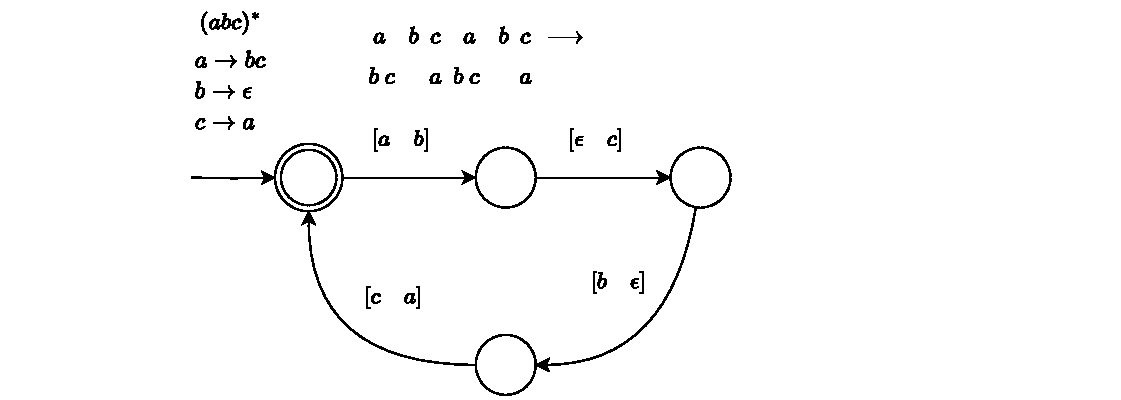
\includegraphics[scale=1.0, keepaspectratio]{obrazky-figures/transducer.drawio.pdf}
  \caption{
    Example of a 2-tape input/output \nft.
  }\label{fig:2_tape_nft}
\end{figure}

\end{example}

\section{Data Structure}
We propose utilizing the existing data structures in \mata (used for NFAs) for implementing finite transducers in \mata.
The main advantage is that NFAs, \nfts, and BDDs can all be implemented using the same single data structure, utilizing a lot of the existing algorithms on the data structures.

\mata provides a base class \nfaClass which encompasses both deterministic and non-deterministic finite automata and operations on them.
Class \nfaClass is a base class from which \nfts, BDDs, and register automata can inherit, including all operations on \nfaClass where only a few specific operations need to be modified for each respective type of finite-state machine.
This hierarchy also allows us to add model-specific operations to each type of automata without modifying operations for the other automata.
BDDs in our representation only extend the functionality of \nfts, and can therefore inherit most of the algorithms from \nfts and only modify some of the algorithms for BDD-specific use-cases.

\begin{figure}[ht]
  \centering
  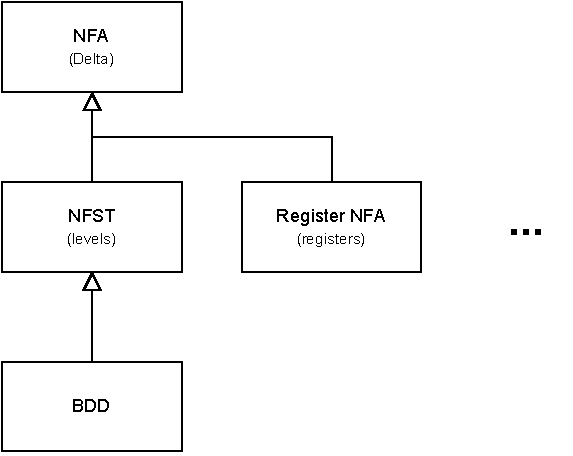
\includegraphics[scale=0.8, keepaspectratio]{jumps_synchronization-NFAs-NFSTs-BDDs-hierarchy.drawio.pdf}
  \caption{
    An inheritance hierarchy for NFAs, \nfts, BDDs, and register automata.
    All of these finite-state machines utilize the same data structure, with mostly the same algorithms where only a few algorithms needs to be modified for each respective type of finite-state machine.
    Each type of finite-state machine can further extend the set of operations by their own specific operations.
    Since BDDs only extend the functionality of transducers, BDDs can inherit directly from \nfts, modifying a few algorithms of \nfts together with the base \nfaClass algorithms.
  }
\end{figure}

Class \nfaClass defines which states in the represented automaton are initial (a set of initial states) and which are final (a set of final states).
Furthermore, \nfaClass allows for storing of arbitraty context in the automaton itself.

The most important data structure for the representation of the finite-state machines and the efficiency of the algorithms run on the representation is the representation of transition relation, called \deltastruct in \mata.
\deltastruct defines the set of states of the finite automaton, and gives the transition relation of the finite automaton.
\deltastruct is designed in such a way that often used operations such as iteration over transitions, adding and removing transitions, are performant, while less often used operations such as reversal of transition relation can be less performant.

States are in \mata represented as unsigned integers, numbered from 0.
This allows adding new states to the automaton to be as easy as getting the number of states in \deltastruct (constant time operation) and adding a number equal to the number of new states we want to add.
Such states are immediatelly allocated in \deltastruct and can be used in initial of final states sets.

Transition symbols are internally stored as unsigned integers as well, numbered from 0, where the last several unsigned integer values are reserved for epsilon symbols.
\mata provides several alphabet types which map the actual transition symbols to their internal values.

The use of unsigned integers for states and symbols gives implicit ordering over both states and symbols and querying them by accessing index corresponding to the internal state/symbol value in an ordered vector.
\deltastruct is a three-level data structure where each level represents one element from the three-tuple $(q, s, q')$ representing a single transition as:
\begin{enumerate}
    \item source states,
    \item transition symbols,
    \item target states.
\end{enumerate}

Each level is internally stored in memory as a sorted vector of unsigned integers, stored in a low-level data structure provided by \mata called \ordvector, a wrapper over \texttt{std::vector} maintaining a set of elements inserted to \texttt{std::vector} ordered.

\ordvector therefore has constant time access to stored elements, operations on the largest element (implemented internally as \texttt{push\_back()}, \texttt{pop\_back()}), fast linear iteration over the elements, and linear union, intersection, and difference.
Since vectors are ordered, lookup for states and symbols is logarithmic using binary search.
Insertion and removal of are logarithmic, but they must shift elements in the memory in the underlying \texttt{std::vector} which slows the operations down.

Due to this, \mata tries to iterate over \ordvector as often as possible since internally, \texttt{std::vector} stores elements in a continuous array on heap with good memory locality, and add elements one after the other in an ascending order given by the value of the inserted elements at the end of the ordered vector.
Several algorithms such as synchronized traversal over multiple ordered vectors.
General insertion and removal of transitions are logarithmic, but \mata algorithms are written in such a way that the general insertion and removal are seldom used.

This pairs well with underlying data structures for sets of initial and final states, implemented as sparse sets~\cite{sparseset93} allowing for constant element lookup, insertion and removal, and fast linear iteration through elements.

The Figure~\ref{fig:delta_struct} visualizes the three-level \deltastruct data structure. We can see that the when we access by source state $q$ the index in the first vector of source states, we get a vector post of type \statepost (\statepost[q]), representing $\post(q)$, which is a vector of symbol posts for each transition symbol $a$ leading from source state $q$, of type \symbolpost.
Each symbol post for symbol $a$ represents $\post(q, a)$, storing the transition symbol $a$ and a set of target states represented as a \ordvector.

% {\tiny
\begin{figure}[ht]
\begin{center}
% \includegraphics[width=10cm]{images/Delta.pdf}
% TODO: Replace with my own image of Delta struct.
\definecolor{color1}{RGB}{54,174,124}
\definecolor{color2}{RGB}{24,116,152}
\begin{tikzpicture}[
    circ/.style={draw,circle,inner sep=0pt,minimum size=2pt,fill},
    arr/.style={->,thick,>=stealth},
    type/.style={color2,dashed,thick},
    % >=stealth,
]

\matrix[
    matrix of nodes,
    nodes={draw, minimum size=5mm},
    % column sep=-\pgflinewidth,
    row sep=0.5mm,
    nodes in empty cells,
    row 1/.style={nodes={draw=none, fill=none, minimum size=5mm}},
% row 1 column 1/.style={nodes={draw}}
] (delta) {
0 & 1 & 2 & 3 & 4 & 5 & 6 & 7 & 8 & 9\\
  &   &   &   &   &   &   &   &   &  \\
};
\node[below = 0cm of delta-2-8,xshift=4.5mm] {\code{std{::}vector{<}StatePost{>}}};
\draw[decoration={brace,amplitude=10pt}, decorate, color1, thick] (delta-1-1.north west) -- (delta-1-10.north east) node [above = 10pt, pos=0.5] {Source states};
\draw[type] plot [smooth,tension=2] coordinates {($(delta.west)+(-2,-5)$) ($(delta)+(0,1.5)$) ($(delta.east)+(2,-5)$)};
\node[right = 1cm of delta,color2] {\code{Delta}};

\matrix[
    matrix of nodes,
    nodes={draw, minimum size=5mm, anchor=center, %text centered, align=center
    },
    % column sep=-\pgflinewidth,
    % row sep=0.5mm,
    % nodes in empty cells,
    below = 1.3cm of delta-2-6
] (statepost) {
$a$ & $c$ & $e$ & $r$ & $x$ & $\epsilon$ \\
};
\draw[arr] ($(delta-2-5.north west)!0.5!(delta-2-5.south east)$) node[circ]{} .. controls +(0,-.7) and +(0,0.7) .. (statepost-1-1.north west);
\node[below = 0cm of statepost-1-5] {\ordvector{}\code{{<}SymbolPost{>}}};
\node[above = 0cm of statepost-1-4, color1] {Transition symbols};
\draw[type] plot [smooth,tension=2] coordinates {($(statepost.west)+(-1.5,-2.5)$) ($(statepost)+(0,1)$) ($(statepost.east)+(1.5,-2.5)$)};
\node[right = 0.8cm of statepost,color2] {\code{StatePost}};

\matrix[
    matrix of nodes,
    nodes={draw, minimum size=5mm, anchor=center, %text centered, align=center
    },
    % column sep=-\pgflinewidth,
    % row sep=0.5mm,
    % nodes in empty cells,
    below = 1.3cm of statepost-1-2
] (symbolpost1) {
1 & 3 & 5 & 6\\
};
\draw[arr] ($(statepost-1-2.north west)!0.5!(statepost-1-2.south east)+(0.17,0)$) node[circ]{} .. controls +(0,-.7) and +(0,0.7) .. (symbolpost1-1-1.north west);
\node[below = 0cm of symbolpost1-1-3] {\ordvector{}\code{{<}State{>}}};
\node[above = 0cm of symbolpost1-1-3, color1] {Target states};
\draw[type] plot [smooth, tension=1.1] coordinates {($(symbolpost1.south west)+(-0.2,0)$) ($(statepost-1-2)+(0,0.15)$) ($(symbolpost1.south east)+(0.2,0)$)};
\node[right = 0.2cm of symbolpost1,color2] {\code{SymbolPost}};

\end{tikzpicture}

\end{center}
% \vspace{-6mm}
\caption{
The vizualization of the three-level data structure representing the transition relation of finite-state machine in \mata, called \deltastruct.
}
\label{fig:delta_struct}
% \vspace{-4mm}
\end{figure}
% }

Notice that since \mata supports epsilon symbols as maximal unsigned integer values, the symbol posts for epsilons are always at the end of state posts and can be therefore accessed in constant time instead of having to search the whole state post to look them up. \mata operations utilize this fact in numerous operations using epsilon symbols such as in string solving~\cite{fm23_equations_synergy_regular_constraints_DBLP:conf/fm/BlahoudekCCHHLS23}.

\nfts and BDDs can directly utilize \nfaClass with all of the underlying data structures where one transition in \nft is represented by several transitions in \nfaClass.
The only modification of \nfaClass to support \nfts and BDDs is adding a vector of state \emph{levels} (represented by \texttt{std::vector}<unsigned>) indexed by automaton states, as in the first level in \deltastruct. The vector maps each aumaton state to its level in the finite-state machine.
$n$-tape \nft has $n$ levels.
Therefore, in a representation of a $n$-tape \nft, vector of state levels maps to values from $0$ to $n-1$.
One transition in \nft corresponds to $n$ transitions in \nfaClass.

Each transition in \nfaClass corresponds to one level of the \nft, i.e., one tape of the \nft.
\nft transition always starts in level $0$. Transition from level $0$ to level $1$ represents the operation on the first \nft tape, from level $1$ to level $2$ the second \nft tape operation and so on.
Finally, the transition from state with level $n-1$ back to state with level $0$ corresponds to the last tape in the \nft.
For 2-tape (input/output) \nft, the levels used will be $0$ and $1$, where transitions from states with levels $0$ represent the ipnut transitions and transitions from states with levels $1$ represent the output transitions.

For this reason, \nfts can have as initial or final states only states with state level $0$.
This is crutial for many algorithms (more in~\ref{sec:Algorithms}) which rely on certain invariants in the representation of \nfts, such as that \nfts always synchronize in states with state level $0$ and each step in operations must consider the entire state levels sequence from $0$ to $n-1$ as a single \emph{abstract} step.

\subsection{Epsilon and Don't Care Transitions}

\nfts and BDDs also need suport for epsilon symbols and don't care symbols on transitions.

\mata already supports epsilon symbols as (several) last transition symbol(s) in the range of possible transition symbols given by the data type of transition symbol.
Adding support for \emph{don't care} symbols on transitions, matching any transition symbol on the tape.

An epsilon symbol on a transition from state with level $k$ to level $k + 1 \% n$ in \nfaClass representing a \nft means that the tape corresponding to the level $k$ does not read from / write on the tape $k$ any symbol.

\nfts represented as \nfaClass also require support for \emph{jumps} where the transition goes from a state with level $k$ to any other state with level $l$ where $l \neq k + 1$.
However, we restrict the jumps for $n$-tape \nft as follows:
\begin{itemize}
  \item The jump cannot jump over a state with level $0$.
  That is, if we need to jump further, the transition can at most jump to the next state with level $0$,
  \item A jump of length $k$ greater than one (the length of one is a normal transition in \nfaClass which we call just a transition) is interpreted the same as if we made $k$ transitions in \nfaClass with the transition symbol on the jump transition.
  That is, a jump of length $3$ (over $3$ tapes) with transition symbol $\epsilon$ means that the transducer made $3$ normal transitions with $\epsilon$ as a transition symbol for each of them.
  \item Jumping from a state with level $0$ to the next state with level $0$ means that only the internal state of the \nft has changed (the state has changed) without reading or writing anything on any of the tapes.
\end{itemize}

% TODO: Figure for jumps.




\begin{example}\label{example:2_tape_nft_in_mata}
  The \nft from Example~\ref{example:2_tape_nft} is represented in the data structure for \nfts inherited from \nfaClass as in the Figure~\ref{fig:2_tape_nft_in_mata}.

  Transitions from states with level $0$ represent the input tape transition symbol, and transitions from states with level $1$ represent the output tape transition symbol.

  \begin{figure}[ht]
    \centering
    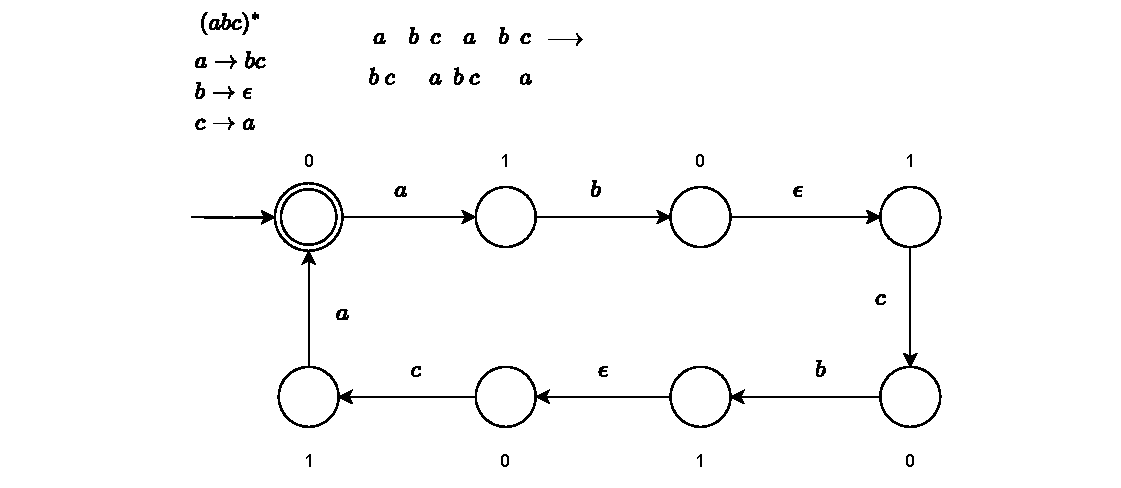
\includegraphics[scale=1.0,keepaspectratio]{obrazky-figures/transducer_in_mata.drawio.pdf}
    \caption{
      2-tape \nft from Example~\ref{example:2_tape_nft} represented in \mata as an \nfaClass with states annotated by state levels.
    }\label{fig:2_tape_nft_in_mata}
  \end{figure}
\end{example}

\subsection{No Operation Transitions}
An epsilon transition from a state with level $k$ to $k+1 \mod n$ can be understood as a \emph{no operation transition} \nop, i.e., a transition where the current tape does not perform any operation (no reading nor writing). In essence the impact of the transition is the same as if reading an empty string on the current tape.

In constrast, an epsilon transition from a state with level $k$ to another state with level $k$ is a simple change of states (as per the usual definition of epsilon transitions in \nfas).

Depending on the application, one might prefer to use one or the other representation as needed.
In this work, we use \nop when we want to explicitly stress the distinction between a simple change of state in \nft (an epsilon transition between states with the same level), and no operation on a current tape (tape does not read nor writes any symbol).

\section{Algorithms}
\label{sec:Algorithms}

For general uses of transducers in \mata, we have implemented general automata operations for creating, modifying, and manipulating transducers.
Furthermore, we have implemented several transducer-specific operations.

\begin{itemize}
  \item Synchronization,
  \item concatenate
  \item get\_one\_letter\_aut
  \item \ldots
\end{itemize}

\subsection{Synchronization}

All operations performing some kind of traversal over the transitions start the compution from states with level $0$.
\nfts are always synchronized on states with level $0$, that is, after each \nft transition is completed (all tape operations are handled).
If the macro-state in a worklist contains only states of multiple \nfts with levels $0$, the \nfts are synchronized and the next macro-state can be computed.
When the synchronized \nfts perform one transition, due to the supported jumps, the new macro state may contain states with different levels.
Only the state in the macro-state with the level furthest behind is expanded.
The others are at least one step ahead and therefore cannot be expanded and must wait for the states behind to get to at least their levels first before being expanded themselves.

Since jumps can jump at most to the next state with level $0$, we always know which states in the macro-state are ahead and which are behind by the following method.
If we expand a macro-state with states with levels $k$ and $l$ where $k > l$, we know that state with level $k$ must be ahead of the state with level $l$.
If any of the states has level $0$ (and there are other states with nonzero levels), we know that the state $0$ must be ahead of all the other states with nonzero levels, and synchronized with all other states with levels $0$.
That holds since the states with levels $0$ can only be the next states with levels $0$, and not the states with level $0$ behind (as the first step from the synchronized states is to move immediately out of the states with level $0$ behind).

The same holds for BDDs utilizing the same data structure and constraints as \nfts.

\begin{example}
  If we perform synchronization over three $4$-tape \nfts, starting from macro-state with levels $(0, 0, 0)$, we perform one transition and may end up in a macro-state with levels $(3, 1, 0)$ where the first \nft made a jump of length $3$, the second performed normal transition (jump of length $0$), and the last \nft performed a jump to the next state with level $0$.
  When expanding the macro-state $(3, 1, 0)$ later on, we know that the state with level $0$ is ahead of the other states with levels $3$ and $1$. And we further know that state with level $3$ must be ahead of the state with level $1$. Therefore, the state with level $1$ must be expanded up until the level reaches $3$ or greater (the next level $0$).
  Then we may get $(3, 3, 0)$, both the first and the second state are expanded to states with levels $(0, 0, 0)$ and the macro-state is synchronized again.
\end{example}

\begin{figure}[ht]
  \centering
  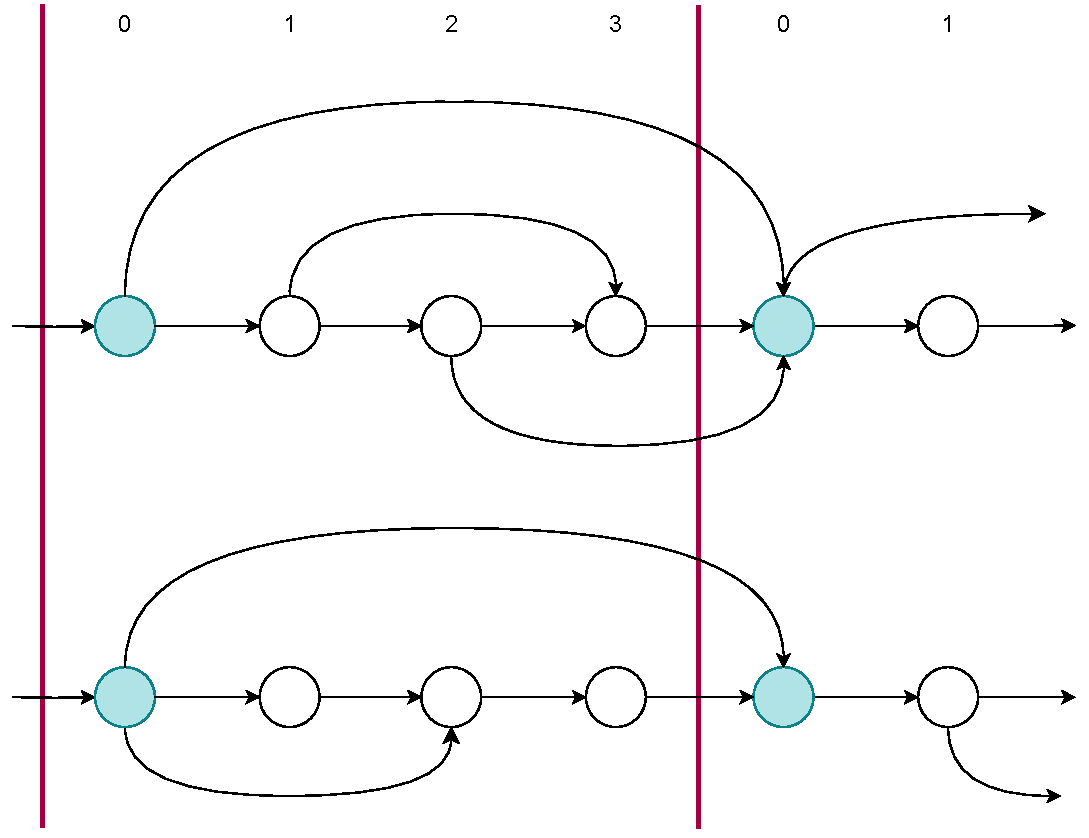
\includegraphics[scale=0.7, keepaspectratio]{obrazky-figures/jumps_synchronization.drawio.pdf}
  \caption{
    An example of allowed jumps in $4$-tape \nfts during synchronization.
    Jumps can start in state with any level and jump up to the next state with level $0$.
    The jumps cannot jump over states with level $0$, however.
  }

\end{figure}


\paragraph{Alternative representation of jumps.}
If the restriction of allowed jumps being only to the next state with level $0$ is too strict, an alternative approach where jumps are allowed to jump over (potentially multiple) states with level $0$ can be chosen.
However, during operations such as product construction, an additional information must be added to the worklist containing macro-states containing a list of lengths of each jump performed during the expansion of the last macro state in order to know how far ahead are the states jumped to in relation to the other states in the macro-state.

We deem this approach inferior to our chosen approach since it distorts the simplicity of a single data structure and algorithms on it for NFAs, \nfts, and BDDs.

% ==================================
\subsection{Projection}

The first standard operation on transducers is \emph{projection}.
Given an $n$-tape \nft $\ft$, we can perform \emph{projection to} a specified set of tapes, or \emph{project out} a specified set of tapes.

The transitions remain the same, the only change is that we remove certain tapes (meaning that for every \nft transition we remove transition symbols on those tapes).
In \mata, this means removing all states with certain levels $k$ and their outgoing transitions and redirecting ingoing transitions to these states to the next states with levels $k + 1 \mod n$ where the outgoing transitions were previously leading to.
This can be iteratively performed on all tapes specified for removal.
When the modification is performed, all remaining levels are shifted toward $0$ to start at $0$ and end with $l - 1$ where $l$ is the new number of tapes remaining in \nft.

Projection to, denoted $\projToSet{M}{\ft}$ where $M \subseteq \{ 0, 1, \ldots, n - 1 \} $ is an operation which removes from $\ft$ all other tapes $o \notin M$ and keeps only those tapes $t \in M$.
In practice, this means that an $n$-tape \nft will be modified into an $|M|$-tape \nft.
If $|M| = 1$, we create a $1$-tape \nft (containing only states with level $0$) which is semantically equivalent to a corresponding \nfa with the same transitions.

Projection out, denoted $\projOutSet{M}{\ft}$, performs the same operation, only now instead of keeping the specified tapes $o \in M$, we remove all tapes $o \in M$, and keep only the tapes $t \in \{ 0, 1, \ldots, n - 1 \} \setminus M$.
If $|M| + 1 = n$, we project out all tapes except for one.
This creates a $1$-tape \nft, which is again semantically equivalent to a corresponding \nfa with the same transitions.

Note that for either variation, removing the first tape in \nft transitions requires setting new initial states (the original targets of transitions from the states with level $0$ become the new initial states).
Similarly, removing the last tape in \nft transitions requires setting new final states (the original source of ingoing transitions to the final states become the new final states).
If jump transitions are involved, one may need to expand the jumps into normal transitions between levels to set the correct initial and final states on the new first and last tape.

\begin{example}
  Given an \nft $\ft$ with $5$ tapes, with levels $\{ 0, 1, 2, 3, 4 \}$.

  We can perform the following operations:
  \begin{itemize}
    \item $\projOutSet{\{ 3 \}}{\ft}$ which deletes tape $3$ from $\ft$, leaving tapes $\{ 0, 1, 2, 4 \}$ which are then renumbered to $\{ 0, 1, 2, 3 \}$.
    \item On the result, we can perform $\projToSet{\{ 1, 3 \}}{\ft}$ which performs the same as if calling $\projOutSet{\{ 0, 2 \} }{\ft}$.
    Tapes $0$ and $2$ are removed, leaving tapes $\{ 1, 3 \}$, which are then renumbered to $\{ 0, 1 \}$.
    \item Now, peforming $\projToSet{\{ 1 \}}{\ft}$ gives us \nft with only one tape, which represents the \nfa for the tape $1$.
    Performing $\projOutSet{\{ 1 \}}{\ft}$ instead would give us \nft with only one tape representing the \nfa for the tape $0$.
  \end{itemize}

\end{example}

% ==================================
\subsection{Intersection}\label{sec:intersection}

For constructing the intersection of two \nfts, we make use of the inheritance of \nfts from \nfas and utilize the classical intersection computation on \nfa using the standard product construction algorithm (as described in Chapter~\ref{sec:Preliminaries}).
The only modification is adding support for proper assignment of levels to new macrostates depending on the levels of the original \nft states in the macrostate, and handling of various combinations of transition symbols during the process of adding transitions leading from the macrostates.

TODO
- should it be its own subsection?
- more of a helper function.
- resulting level of a macrostate due to the different orig state levels
- special handling of combinations of symbols.
  - process epsilons
  - process dont\_cares

% ==================================
\subsection{Composition}

When working with \nfts as transduction machines taking some input, modifying it and outputting some output, we often encounter problems where we want to perform multiple transductions on the input, one after the other.
In the same way as we can compose mathematical functions $(f \circ g)(x)$ meaning $f(g(x))$ (perform $g$ on $x$ and perform $f$ on the result of $g(x)$),
we can perform multiple \nfts transductions sequentially: $\ft_2 \circ \ft_1$
(perform the transduction of $\ft_1$ on the input, and then perform the transduction of $\ft_2$ on the result), denotes as $\compose{\ft_1}{\ft_2}$.
Using the Unix \emph{pipe} notation, we can express the same with $\ft_1 \composePipe \ft_2$
(perform the transduction of $\ft_1$ on the input, and then pipe the result to $\ft_2$ to perform the transduction of $\ft_2$ on the result).

\begin{example}
  Throughout this section, we will demonstrate the composition algorithm on the following example.
  Given \nft $\ft_1$ with tapes $0$, $1$, and $2$, and $\ft_2$ with tapes $2$, $3$, $4$, we want to compute $\ft_1 \composePipe \ft_2$, synchronizing both \nfts on tape $2$.
  For clarity, we number the tapes uniquely between both \nfts in this example. Internally, each \nft has tapes with levels from $0$ to $2$ and for each \nft, we specify which tape(s) the \nfts should synchronize on.
\end{example}

The composition comprises the following steps:
\begin{itemize}
  \item Extending the \nfts to contain matching tapes,
  \item adding special self-loops on states with level $0$ to allow for proper handling of $\epsilon$ and $\dontCare$ symbols on the transitions,
  \item Performing \nft intersection as described in Section~\ref{sec:intersection}, and
  \item projecting out the synchronization tapes (as described in Section~\ref{sec:projection}) which were "consumed" by the composition.
\end{itemize}

\paragraph{Extending \nfts to match each other.}
The first step of the composition is to extend the input \nfts by inserting additional levels $k$ (additional states with levels $k$) into each transition with $\dontCare$ symbols on the transitions at levels $k$.
This operation balances out the \nfts so both have the same tapes in the same order.
This allows us to perform the classic \nfa intersection for each level in both \nfts during \nft intersection.

\begin{example}
  Continuing the example, we extend each \nft transition in $\ft_1$ with $\dontCare$ transitions from existing states with level $2$ to new states with levels $3$, from states with levels $3$ to new states with levels $4$, and finally from states with levels $4$ to the next existing states with levels $0$ (finishing the original \nft transition) which were the original targets of transitions from states with levels $2$.

  Figure~\ref{fig:composition_nfts_extension} shows a depiction of a single transition in $\ft_1$ and $\ft_2$ before and after extension.

  \begin{figure}[ht]
    \centering
    \subfloat[\centering Before extension\label{fig:composition_nfts_extension_before}]{{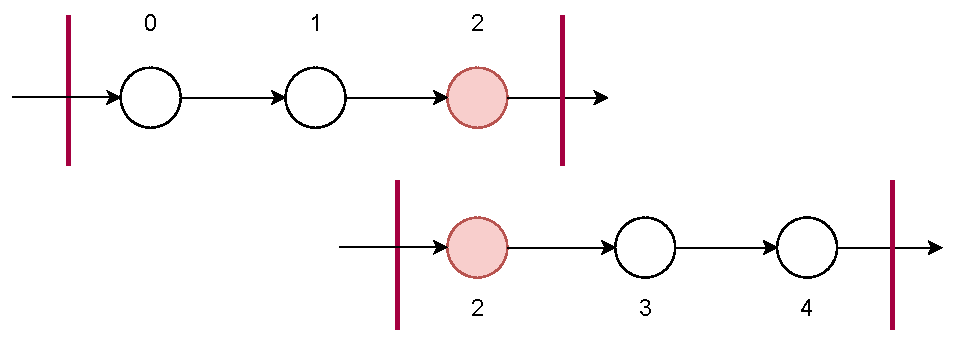
\includegraphics[keepaspectratio,width=0.45\textwidth]{jumps_synchronization-composition_nfts_extension.pdf} }}%
    \qquad
    \subfloat[\centering After extention\label{fig:composition_nfts_extension_after}]{{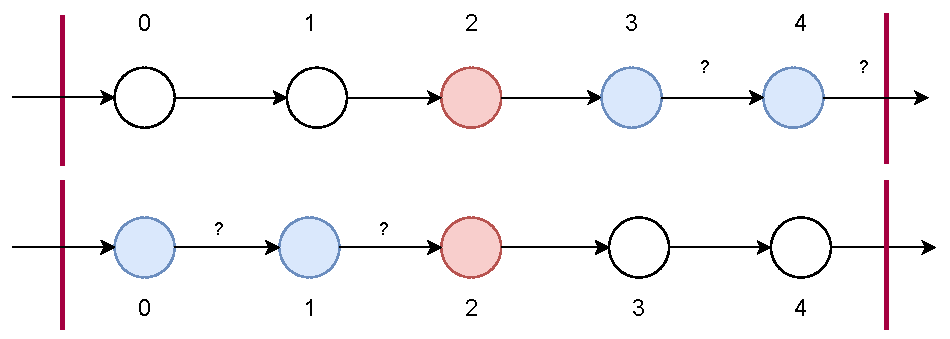
\includegraphics[keepaspectratio,width=0.45\textwidth]{jumps_synchronization-composition_nfts_extension_balanced.pdf} }}%
    \caption{
      A depiction of a single transition in \nfts $\ft_1$ (top) and $\ft_2$ (bottom) before extension (Figure~\ref{fig:composition_nfts_extension_before}) and after extension with $\dontCare$ transitions on inserted tapes to balance out the tapes in both \nfts (Figure~\ref{fig:composition_nfts_extension_after}).
      The red states with together with the outgoing transition represent the tape $\ft_1$ and $\ft_2$ are synchornized on.
      The blue states represent the newly inserted tapes with $\dontCare$ symbols on transitions.
    }
    \label{fig:composition_nfts_extension}%
  \end{figure}

  We can see that after the extension, both $\ft_1$ and $\ft_2$ have the same tapes.
\end{example}

Thanks to this general approach, we can compute compositions of any $n$-tape \nfts\footnote{Where $\ft_1$ and $\ft_2$ does not even have to have the same $n$.}, synchronizing on any tape(s)\footnote{When synchronizing on multiple tapes, the tapes must at least be in the same order in both \nfts.}, with the tapes being in an arbitrary order.

As an optimization, when adding multiple subsequent $\dontCare$ transitions during the extension, we can instead add only a single $\dontCare$ jump from the first state in the sequence leading to the last state in the sequence, without having to create new states for all inserted tapes being jumped over.

\paragraph{Adding self-loops.}
The next step is to add self-loops to all states with level $0$ in both \nfts.
These self-loops serve the purpose of nondeterministic "waiting" loops for waiting at the beginning of an \nft transition in one \nft for the other \nft to

\paragraph{Intersection.}
When the \nfts are balanced out and self-loops are added, we can perform an \nft intersection, as per Section~\ref{sec:intersection}.
The intersection produces a new \nft representing the composition of $\ft = \ft_1 \composePipe \ft2$, only currently $\ft$ still contains all the tapes from the balanced $\ft_1$ and $\ft_2$.
Other that that, the composition is complete.

\paragraph{Projecting out the tapes the composition synchronized on.}
To clean up $\ft$, we need to project out the tapes we synchronized on as these are the tapes that have been "consumed" by the composition.

TODO
- perform intersectoin
- project out the levels used to synchronize on.

For working with only $2$-tape \nfts, a spe|alized, more performant algorithm for composition could be utilized.
The algorithm would still utilize the general idea of \nft intersection, but now no extension of \nfts and no self-loops are necessary.
For each macrostate, we would first perform a step in $\ft_1$ on level $0$, then perform the synchronized step on levels $1$ in $\ft_1$ and $0$ in $\ft_2$ (if such a step is possible as per \nft intersection rules), then finish the composition of the current transition by performing a step in $\ft_2$ on level $1$, constructing a new macrostate from targets of transitions on levels $1$ of both \nfts.
Handling of jumps is similar to \nft intersection: waiting for the state "left behind" to catch up with the state jumped to.

% ==================================
\subsection{Application}

When we construct an \nft $\ft$, the most intuitive use of $\ft$ is to perform the transduction (the process of reading the input on input tapes and outputting the output on the output tapes) $\ft$ encodes.
This operation is called \emph{Application}.

We can \emph{apply} a word $w$ on $\ft$, or a regular language $\langof{\aut}$ for some $\aut$.

\paragraph{Application of a word.}
We can either apply a word $w \in \Sigma^*$ on a given tape (at level $k$), or apply an $l$-tuple of words $(w_i)$ where $i in \in \{ 1, \ldots, n \}$ where $|(w_i)| = l$ and $i$ specifies on which tapes we want to apply the tuple of words (one word $w_i$ for each tape $i$).

The result of the application of a word (or a tuple of words) is a set of tuples of size $(n - l)$ of words.
We read the word(s) being applied and move through the \nft according to the transition symbols in the applied word(s) on the corresponding tapes, similarly to performing a run on a word in \nfa, only now to potentially multiple tapes (multiple words).
During the traversal, we construct the result by appending the transition symbols on the remaining tapes to the result constructed so far for the current state.
This gives us the corresponding word on the remaing tapes when the words on the given tapes are $(w_i)$.

Focusing on $2$-tape \nfts $\ft$, the application equals to translation from the input word $w$ to the output word $w'$ (similarly to what a natural language translator does) where $w' = \apply{\ft}{w}$.
By convention, we presume the input tape is at level $0$ and the output tape is at level $1$.

The application of a word is equivalent to $\idNft{\aut} \composePipe \ft$ where $\aut$ represents a \dfa accepting only $w$.
This gives us an \nft encoding the result.
For $2$-tape $\ft$, we get a $1$-tape \nft, equal to the corresponding \nfa encoding the set of words in the result.

\paragraph{Application of a language.}
Applying a regular language $\langof{\aut}$ on $n$-tape \nft $\ft$ instead of a single word is performed similarly to the application of a single word, but now the result is a regular language (for $2$-tape \nfts) or an \nft $\ft'$ with $n-1$ tapes.

The application of a language $\langof{\aut}$, similarly to the application of a word, is equivalent to $\idNft{\aut} \composePipe \ft$.
The resulting \nft encodes the result.
For $2$-tape $\ft$, we get a $1$-tape \nft, equal to the corresponding \nfa encoding the regular language of the result.



% Basic approach, operations, representation
\chapter{Finite Transducers for String Solving}

SMT String solving is a complex and diversive problem which has seen a lot of interest over the past few decades.
Many different approaches for reasoning about word equations, word disequations, regular constraints, and length constraints have emerged, be it as a theoretical work, or implemented directly in one or more of the current state-of-the-art SMT string solvers, e.g., ~\cite{cvc4,cvc5,z3,Z3-str,Z3Str3,Z3str4,Trau,fm23_equations_synergy_regular_constraints_DBLP:conf/fm/BlahoudekCCHHLS23, tacas24_noodler_10.1007/978-3-031-57246-3_2, oopsla23_stabilization_DBLP:journals/pacmpl/ChenCHHLS23}.
Each invented approach and each string solver brings a unique set of features and advantages.

We decided to try a novel approach in \noodler, entirely different from other state-of-the-art SMT string solvers (except for \ostrich).
\noodler utilizes finite automata to encode the SMT formulae into a set of regular language constraints where the operations on finite automata as well as the representation of the finite automata themselves is handled by \mata.
This approach gives \noodler a unique oportunity to efficiently encode several problems in string solving as operations on finite automata which other string solvers cannot utilize.

Finite automata can encode regular languages, but string solving problems work with various SMT operations, where some of them cannot be easily encoded into only regular languages.
Such examples are regular replacement operations, namely \texttt{str.replace}, \texttt{str.replace\_re}, \texttt{str.replace\_all} and \texttt{str.replace\_re\_all} from the theory of strings in SMTLIB~\cite{smtlib_theory_strings}.
However, finite transducers naturally encode rational relations between regular languages which can be directly utilized to encode such problematic SMT operations while allowing for efficient automata (transducer) operations on the relations and languages.

If \noodler could utilize finite transducers in a similar fashion to how it utilizes finite automata in its decision procedure, these SMT operations would be easy to compute and integration of finite transducers into its decision procedure would be a natural extension of the existing decision procedure.

Thus, we discuss in this chapter how to utilize finite transducers in \noodler to solve SMT string constraints \texttt{str.replace}, \texttt{str.replace\_re}, \texttt{str.replace\_all} and \texttt{str.replace\_re\_all}.

\section{Replace Operations}
A general regular replacement operation has the following form:
\begin{center}
\begin{verbatim}
  replaced_string = replace(input_string, pattern, replacement)
\end{verbatim}
\end{center}
where \texttt{replace} determines the type of the regular replacement (the semantics of the replacement operation).
\texttt{input\_string} represents the original input string where we want to replace some regular \texttt{pattern} with a \texttt{replacement} literal.
Regular \texttt{pattern} can be a string literal (a word) or a regular language describing the substring (or substrings) of \texttt{input\_string} we are trying to replace.

There are various replacement semantics for replace operations. Popular regular replacement types are \emph{reluctant replacement}, \emph{greedy replacement}, or \emph{possessive replacement}, or \emph{declarative replacement}.
For example, reluctant replacement matches a given \texttt{pattern} (a regular language) with the shortest substring of the \texttt{input\_string}, while the greedy replacement matches the longest substring. These types produce the same result when \texttt{pattern} is a string literal.
Possessive replacement semantics is that of the greedy one, but without backtracking on the substring matched so far.
Declarative replacement matches every occurrence of regular \texttt{pattern} in the given \texttt{input\_string}.

In opposition, \emph{procedural} regular replacements encompass the greedy and reluctant replacements since both match in \texttt{input\_string} from the left to the right.
The start with the first character in the word and by using backtracking continue through the word until the end of the word.

Since SMT-LIB defines only replacement operations of type reluctant replacement with the left-most matching and other types of the replacement operations are not allowed in SMT formulae in SMT-LIB format (which \noodler solves), we focus in this work solely on the reluctant replacement type.

We denote reluctant regular replacement as $x_{\pi \rightarrow y}$ as where $x$ is the \texttt{input\_string}, $\pi$ is the regular \texttt{pattern} (a literal or a regular language) and $y$ is the \texttt{replacement}.

\section{Encoding Reluctant Regular Replacement as Finite Transducers}

SMT-LIB suports two types of reluctant replacements: a \emph{reluctant all replacement} which replaces all occurrences of the shortest left-most matches of \texttt{pattern}, and \emph{reluctant single replacement} which replaces only the first shortest left-most occurrence of \texttt{pattern}.

\paragraph{Epsilon in \texttt{pattern}.}
If the \texttt{pattern} contains epsilon symbol, a special handling of epsilon matching needs to be performed. In such a case, one encodes the replacement operation as if $\epsilon \notin \pi$, and solves the replacement for two options:
\begin{itemize}
  \item Tries solving for just $\epsilon$ manually, and alternatively
  \item Solves the reluctant replacement without the epsilon if the $\epsilon$ match fails.
\end{itemize}
Since SMT-LIB works only with reluctant replacements, the reluctant replacement would always pick the shortest replacement, i.e., the $\epsilon$ replacement. The reluctant match of $\epsilon$ will always succeed and longer matches will not be needed nor accepted. SMT-LIB declares results to such patterns with $\epsilon$ to be equal to $\texttt{replacement} \concat \texttt{input\_string}$ (prepending the replacement to the \texttt{input\_string}).

% Define reluctant replacement.

\begin{definition}[\textbf{Reluctant all replacement}] \hfill \newline
  A \emph{reluctant all replacement} $x^{+}_{\pi \rightarrow y}$ is defined as follows: \newline
  $$x^{+}_{\pi \rightarrow y} = \{ u \concat y \concat w^{+}_{\pi \rightarrow y} \} \text{,}$$
  where $u, v, w, x, y \in \Sigma^*$, $\pi$ is a regular language (regex), $x = u v w$, $u \notin \Sigma^* \pi \Sigma^*$, $v \in \pi$, and to ensure the shortest left-most matching, the following must hold: $\forall u = u_1 u_2, v = v_1 v_2, w = w_1 w_2:$ if $v_2 \neq \epsilon$ then $v_1 \notin \pi$ (the shortest match as if $v_1$ is not a match, then surely the  shortest match is $v = v_1v_2$); if $u_2 \neq \epsilon$ then $u_2 v_1 \notin \pi \land u_2 v w_1 \notin \pi$ (the left-most match is $v$ since there is no match of $\pi$ before $v$).
\end{definition}

A reluctant single replacement is defined similarly, only the recursive replacement of $w$ is no longer performed since after the first replacement of $v$, no more patterns matchings are tried on the substring $w$ after the replaced substring $v$.
\begin{definition}[\textbf{Reluctant single replacement}] \hfill \newline
  A \emph{reluctant single replacement} $x^{1}_{\pi \rightarrow y}$ is defined as reluctnant all replacement, only with the recursive replacement removed:
  $$x^{1}_{\pi \rightarrow y} = \{ u \concat y \concat w \} \text{.}$$
\end{definition}

\begin{example}
  For $a, b, c \in \Sigma$: $aabaaba^{+}_{aa \rightarrow c} = \{ cbcba \}$; $aabaaba^{1}_{aa \rightarrow c} = \{ cbaaba \}$;
\end{example}

\section{Finite Transducer for Regex Reluctant Replacement}

First, we introduce a method for constructing a finite transducer $\ftRegexRelucAll$ for the most general case of reluctant regular replacement, a \emph{regex reluctant all replacement} $x^{+}_{\pi \rightarrow y}$, where the pattern $\pi$ being replaced is specified as a regular language and we replace all occurrences of $\pi$.

We follow the idea of the existing procedure for constructing \nft for regex reluctant all replacement operation taken from~\cite{replace_nfts_model_ModelingRegularReplacementForStringConstraintSolving_DBLP:conf/nfm/FuL10}, but we modify the method to fit SMT-LIB requirements for replacement operations and our implemented representation of \nfts in \mata.

The approach constructs two main \nfts where one non-deterministically finds a possible beginning of a pattern match and inserts a special symbol $\marker$ at the found location in the input word $x$. The symbol $\marker$ serves as a \emph{begin marker} for the searched pattern.

Since we have a reluctant replacement matching the shortest left-most pattern, we know that when we insert the correct begin marker into the input word(followed by a patter match), we can simply read the characters following $\marker$ until we read a matching pattern. There is no need for us to explicitly mark the end of the pattern with another special symbol.\footnote{
  This would not be the case for, e.g., the greedy replacement, however.
}

However, in order to construct the \nft for the begin marker, we first construct a \dft to find a possible \emph{end marker} $\marker$\footnote{For simplicity, we use the same symbol to denote both the begin marker and the end marker. Reason for this is that these two marker are never used simultanously and there is a close connection between them. The connection will be further explained later.} which denotes the end of a pattern, but we construct the \nft the reverse of the searched pattern $\pi$, $\reverse{\pi}$.
This way, we deterministically find the ends of the reversed $\reverse{\pi}$, which gives us the potential beginning of the reverse of $\reverse{\pi}$, that is, the original $\pi$ in $x$.

We will explain the construction on a running example.
Given $x^{+}_{\pi \rightarrow y}$ where $\pi = a^+b^+c$ and $y = d$, construct $\ft_{x^{+}_{\pi \rightarrow y}}$.

\subsection{End Marker \dft}
Here, we construct a \dft $\ftEndMarker$ marking the end of a regular pattern $\reverse{\pi}$.

First, we construct \dfa $\aut_{\reverse{\pi}}$ for $\reverse{\pi}$.
Note that here we treat $\epsilon$ as a special transition symbol used in the construction of $\ftRegexRelucAll$.
Hence, $\aut_{\reverse{\pi}}$ cannot contain $\epsilon$ symbols.
Also note that we require $\aut_{\reverse{\pi}}$ to be deterministic.

See Figure~\cite{fig:end_marker_dfa} for \dfa $\aut_{cb^+a^+}$ for $\reverse{\pi} = cb^+a^+$.

% TODO: Figure.
\begin{figure}[ht]
  \centering
  \caption{\dfa $\aut_{cb^+a^+}$.}
  \label{fig:end_marker_dfa}
\end{figure}

$\aut_{\reverse{\pi}}$ accepts $\reverse{\pi}$, but for replace operations, we need the $\ftRegexRelucAll$ to read any $x \in \Sigma^*$ and replace only the requested pattern, leaving the rest of $x$ unmodified.
Therefore, we \emph{generalize} $\aut_{\reverse{\pi}}$, producing $\aut^{\text{gen}}_{\reverse{\pi}}$, which accepts any word $x \in \Sigma^*$.
Think of $\aut^{\text{gen}}_{\reverse{\pi}}$ as the input tape of an \nft which needs to read any word on its input, and only perform a specific operation (replacement here) for a specified pattern in the input word.

Given $\aut_{\reverse{\pi}} = (\states, \Sigma, \post, \{ q_0 \}, \finalStates)$, we construct $\aut^{\text{gen}}_{\reverse{\pi}} = (\states^{\text{gen}}, \Sigma, \post^{\text{gen}}, { s_0 }, \finalStates^{\text{gen}})$ where $\states^{\text{gen}} = \{ t \,\mid\, t \subseteq \states \}$ following these rules:\newline
We define a bijective mapping $\mathcal{M}: \states^{\text{gen}} \rightarrow 2^{\states }$ such that $\forall s \in \states^{\text{gen}}, a \in \Sigma: s' \in \post^{\text{gen}}(s, a)$
iff $\mathcal{M}(s') = \{ q_0 \} \cup \{ q' \,\mid\, \exists q \in \mathcal{M}(s): q' \in \post(q, a) \}$
and $\mathcal{M}(s_0) = \{ q_0 \}$.

Intuitively, we construct a new \dfa from $\aut_{\reverse{\pi}}$ where each state $s$ maps to a set of states in $\aut_{\reverse{\pi}}$ which can be reached from $q_0$ with the same substrings of $\langof{\aut_{\reverse{\pi}}}$.
Since $\aut_{\reverse{\pi}}$ is deterministic, each substring will end in at most one state $s$.
Thus, $\aut^{\text{gen}}_{\reverse{\pi}}$ remains deterministic.

However, when we encounter state $s$ where $\finalStates \cap \mathcal{M}(s) \neq \emptyset$, we know that we have reached a state in the constructed $\aut^{\text{gen}}_{\reverse{\pi}}$ where the substring corresponding to $s$ is accepted by $\aut_{\reverse{\pi}}$.
That means that we have reached an end of an accepted word in $\aut_{\reverse{\pi}}$ which we want to mark (insert an end marker $\marker$ after this substring).
Therefore, we during the construction, we create a new final state $s_f$, and each time we encounter such a state $s$, we add a transition $\move{s}{\epsilon}{s_f}$, and redirect all transitions which would normally go from $s$ to start in $s_f$.
Thus the only outgoing transition from $s$ is the epsilon transition and we did not introduce a non-determinisctic choice of transition from $s$.
Then, all states except for states $s$ where $\finalStates \cap \mathcal{M}(s) \neq \emptyset$ are made final since we want to accept any arbitrary input.
We omit the original final states since reaching these states is a significant event in reading an arbitrary input which we need to handle separately.

$\aut^{\text{gen}}_{\reverse{\pi}}$ represents an \dfa which states how "far" into $\reverse{\pi}$ we are when reading an arbitrary input.
Each symbol either resets the \dfa (simulating manual backtracking) to some previous matched state or all the way up to $s_0$ (no even partial match was found, we start from the beginning of the pattern), or advances to the next state in the \dfa following the pattern.

Now, $\aut^{\text{gen}}_{\reverse{\pi}}$ accepts any string $x$ on its input.
During the run of $x$ on $\aut^{\text{gen}}_{\reverse{\pi}}$, each time an end of a substring $x_2$ where $x_2 \in \reverse{\pi}$ and $x = x_1 x_2 x_3$ is encountered, an epsilon transition is taken.
If we were to insert $\marker$ into $x$ each time an epsilon transition is taken, we would modify $x$ in such a way that the word would remain the same, only interspersed with $\marker$ after each end of $x_2$ (since $\aut^{\text{gen}}_{cb^+a^+}$ is deterministic, no other transition can be taken from the source state of the epsilon transition).
These $\marker$ represent the end markers we want to insert with $\ftEndMarker$.

See Figure~\cite{fig:generalized_end_marker_dfa} showing a generalized modification of \dfa $\aut_{cb^+a^+}$, $\aut^{\text{gen}}_{cb^+a^+}$.
For example, a word $cbcbba\marker a\marker a\marker bcb$ would be accepted by this automaton where the imaginery string symbol $\marker$ symbolically represents places where an epsilon transition was taken in the automaton.

% TODO: Figure.
\begin{figure}[ht]
  \centering
  \caption{\dfa $\aut^{\text{gen}}_{cb^+a^+}$, a generalized version of $\aut_{cb^+a^+}$.}
  \label{fig:generalized_end_marker_dfa}
\end{figure}

Next, we can construct $\ftEndMarker$ from $\aut^{\text{gen}}_{\reverse{\pi}}$.
We simply consider the current transitions as the input tape of $\ftEndMarker$,
and we add transition symbols for output tape: for all $a \in Sigma$, the  symbol on the output tape is $a$ again, only for input symbol $\epsilon$, the output symbol is $\marker$.

We can see the final $\ftEndMarker$ for $\aut^{\text{gen}}_{cb^+a^+}$ in Figure~\ref{fig:generalized_end_marker_dft}.
\begin{figure}[ht]
  \centering
  \caption{\dft $\ftEndMarker$ for $\aut^{\text{gen}}_{cb^+a^+}$ inserting the end markers $\marker$ at the correct locations in the read input word.}
  \label{fig:generalized_end_marker_dft}
\end{figure}

\subsection{Begin Marker \nft}
We could start constructing the \emph{begin marker} \nft $\ftBeginMarker$ from $\ftEndMarker$ by reversing all transitions in $\ftEndMarker$.
However, considering reversing a single transducer transition (consisting of operations on the input and output tapes), represented as a sequence of two \nfa transitions in \mata from state with level $0$ to $1$ and back to some state with level $0$, we instead utilize $\aut^{\text{gen}}_{\reverse{\pi}}$ before its conversion to $\ftEndMarker$ (and $\ftEndMarker$ is therefore never truly constructed in \mata).

We reverse all transitions in $\aut^{\text{gen}}_{\reverse{\pi}}$, effectively obtaining the foundation for an \nfa for marking beginnings of $\pi$.
We can now construct $\ftBeginMarker$ the same way as we constructed $\ftEndMarker$ from $\aut^{\text{gen}}_{\reverse{\pi}}$ except now $\marker$ as the output symbol for the epsilon symbol on the input tape represents the begin marker instead of the end marker.
This step shows why we use the same marker for symbols for both the begin and end marker.
They mark the same location, only once operating on $\reverse{\pi}$, then on $\pi$.

However, marking beginnings is non-deterministic operation since we cannot know in advance whether the currently read symbol in an arbitrary input string marks a beginning of a full match in $\pi$.
Henceforth, we have introduce another source of non-determinism, which gives us the smart "look-ahead" ability for marking beginnings for only those inputs that will later on truly match in $\pi$.
All potentially incorrectly inserted begin markers in the input word end in a non-accepting run for the word with such begin markers.
We add a new initial state $s'_0$ and add an epsilon transducer transition $\move{s'_0}{\epsilon}{s}$ ($\epsilon$ as the transition symbol on all tapes) leading to all states $s$ which are final in $\aut^{\text{gen}}_{\reverse{\pi}}$, that is, all except those which map to set of states containing the original final state from $\aut_{\reverse{\pi}}$.
The previous initial state of $\ftBeginMarker$ is set as the only final state and is removed from the initial states.

The Figure~\ref{fig:begin_marker_nft} shows a $\ftBeginMarker$ for $\reverse{\aut^{\text{gen}}_{cb^+a^+}}$.
\begin{figure}[ht]
  \centering
  \caption{\nft $\ftBeginMarker$ for $\reverse{\aut^{\text{gen}}_{cb^+a^+}}$ inserting non-deterministically the begin markers $\marker$ at the beginning of matches in $a^+b^+c$ for the read input word.}
  \label{fig:begin_marker_nft}
\end{figure}

\subsection{Reluctant Replacement \nft}

When we have the begin marker \nft $\ftBeginMarker$, we can construct the second \nft performing the actual replacement.
These two \nfts are used to finally construct the whole $\ftRegexRelucAll$.

We already can non-deterministically find the correct begin markers, but we now need to perform the actual replacement(s) on the input string annotated with begin markers.

We construct an \nft $\ftRegexRelucReplaceAll$ which models the actual reluctant replacement.
The idea is that we read the input string annotated with begin markers and output the same symbols unmodified on the output tape.
Once we encounter the begin marker, we know we have found the first left-most match which needs to be replaced.
Therefore, we switch to a "replacement" mode where we read the match without outputting anything, removing all symbols of the match and all additional begin markers inside the match.
Afterwards, the match is read and we can insert the replacement for the match onto the output tape.
When the replacement is inserted, we return to the beginning to potentially perform replacement on another match.

First, we convert the $\aut_{\pi}$ into a new \nfa $\aut^{\text{short}}_{\pi}$ which accepts (matches) only the shortest input words.
This can be easily performed by removing all outgoing transitions from all final states in $\aut_{\pi}$.
Clearly, $\langof{\aut^{\text{short}}_{\pi}} = \{ u \in \langof{\aut_{\pi}} \,\mid\, \neg \exists u' \in \langof{\aut_{\pi}}^{<|u|} \}$.

$\aut^{\text{short}}_{\pi}$ now matches the shortest words in the language of $\aut_{\pi}$, but does not allow skipping over additional $\marker$ encountered during reading the match.
Such $\marker$ need to be skipped since $\marker$ inside the shortest left-most match represent beginnings of potential matches further to the right than the left-most match.
We need to therefore add a self loop to every state in $\aut^{\text{short}}_{\pi}$ with transition symbol $\marker$.

Now the final modification is to keep the next begin marker for the next shortest left-most match. $\aut^{\text{short}'}_{\pi}$ can be constructed given $\Sigma^*_\marker = \Sigma^* \cup \{ \marker \}$ as $\aut^{\text{short}'}_{\pi} = \aut^{\text{short}}_{\pi} \cap \overline{\Sigma^*_\marker \concat \{ \marker \}}$.

$\aut^{\text{short}'}_{\pi}$ can be converted into $\ft^{\text{short}'}_{\pi}$ where the existing transitions are the input tape transitions, and the output symbols are all $\epsilon$ (\nft only reading the input word---the match---and consuming the whole match including $\marker$ inside the match).

Figure~\ref{fig:ft_regex_reluc_replace_all} symbolically shows how to construct $\ftRegexRelucReplaceAll$ for replacing all shortest left-most occurrences of regular language $\pi$ with $y$.

To replace only one occurrence (the first shortest left-most match), a variation of $\ftRegexRelucReplaceAll$, $\ftRegexRelucReplaceSingle$ can be constructed, as seen in Figure~\ref{fig:ft_regex_reluc_replace_single}.
Here we do not return to the beginning after the first replace, but move to a new state with just reads the rest of the word unmodified while removing the additional $\marker$.

\subsection{Whole Regex Reluctant Replace \nft}

We have constructed $\ftBeginMarker$ to insert non-deterministically begin markers into the input word and constructed $\ftRegexRelucReplaceAll$ (or $\ftRegexRelucReplaceSingle$) to perform the replacement upon encountering matches prepended with $\marker$.
$\ftRegexRelucAll$ (and similarly $\ftRegexRelucSingle$) can be constructed by connecting these two \nfts into a sequence using composition: $\ftRegexRelucAll = \ftBeginMarker \composePipe \ftRegexRelucReplaceAll$ and $\ftRegexRelucSingle = \ftBeginMarker \composePipe \ftRegexRelucReplaceSingle$.
$\langof{\ftRegexRelucAll} = \{ (u, v) \in \Sigma^* \,\mid\, v = u^{+}_{\pi \rightarrow y} \} $ and $\langof{\ftRegexRelucSingle} = \{ (u, v) \in \Sigma^* \,\mid\, v = u^{1}_{\pi \rightarrow y} \} $.

\section{Finite Transducer for Literal Reluctant Replacement}

Constructing \nfts for regex reluctant replacement is expensive.
Therefore, when the \texttt{pattern} to be replaced is of a simpler form, namely a string literal, or even a single symbol, a corresponding \nft for reluctant replacement can be constructed faster.

\subsection{Single Symbol Replacement}

We can construct a replacement \dft for a single symbol reluctant replacement by creating a single-state \dft with $\id{\Sigma}$ self-loop transducer transitions.
Then only modify the output transitions for the input symbol to be replaced with to produce the replacement.
The handling of single and all reluctant replacement variations is the same as for regex reluctant replacement.

The Figure~\ref{fig:single_symbol_replacement} shows single symbol replacements for both the single and all replacement variations for replacement being a single symbol and a literal.

\subsection{Replacement of Finite Literal}

To construct a \nft for the replacement of a string literal $z$ with $y$, we need to construct two \nfts.

First, we want to annotate the end of the input words $x$ simlarly to how $\ftEndMarker$ annotates the end of the patterns, but now a simple \nft $\ft_\marker$ with an initial state $q_0$, final state $q_f$, and transitions $(q_0, \id{\Sigma}, q_0)$, and $(q_0, (\epsilon, \marker), q_f)$ will suffice.
$\langof{\ft_\marker} = \Sigma^* \concat \{ \marker \}$.

Second, we need to construct an \nft $\ftLiteralRelucReplaceAll$ for replacing all literals, or $\ftLiteralRelucReplaceSingle$ for replacing only the first left-most shortest literal.

$\ftLiteralRelucReplaceAll = (\states, \Gamma, \post, \{ q_0 \}, \{ q_f \})$ can be constracted using the following method.
We construct a \nft for $z$ where $z$ represents the input tape and a sequence of $\epsilon$ symbols represents the corresponding output tape.
Each state $q$ uniquely maps to its corresponding substring of $y$: $\mathcal{M}: \states \rightarrow \Sigma^*$ is a bijection where $\mathcal{M}(q_0) = \epsilon$, $\mathcal{M}(q_1) = y[0:1]$, $\mathcal{M}(q_1) = y[0:2]$, $\mathcal{M}(q_2) = y[0:3]$, etc.
Each state therefore represents a "buffer" of symbols read so far on the input tape which have not been outputted on the output tape yet.
We already have transitions as constructed from $z$ for each state.

Now we add additional transitions as follows:\newline
\begin{itemize}
  \item If $\marker$ is read on the input tape, we output the contents of the buffer $\mathcal{M}(q)$ where $q$ is the current state (symbols read from the input word but not outputted onto the output tape yet) and move to $q_f$.
  When we succeed by locating prefix starting at index $i$, we split $\mathcal{M}(q) \concat a$ into $l$ and $r$, where $l = p[0:i]$ and $r = p[i:|p|]$.
  We output $l$ onto the output tape (as a sequence of transition symbols) and move to state $q' = \mathcal{M}(r)$ which reprents the longest prefix of $y$ currently being "buffered" and not processed yet.
  \item If $a \in \Sigma, z = \mathcal{M}(q)\concat a$ ($a$ is the last symbol in $y$), we perform the replacement: outputting $y$, and move to the beginning $q_0$ to continue replacing the next matches.
  \item If $a \in \Sigma, a \neq z[|\mathcal{M}(q)|:|\mathcal{M}(q)| + 1]$ ($a$ is not the next symbol in $z$---those transitions are already in  $\ftLiteralRelucReplaceAll$), we determine the longest prefix $p$ of $z$ from $\mathcal{M}(q) \concat a$ from left to right.
\end{itemize}

When constructing $\ftLiteralRelucReplaceSingle$, instead of moving to $q_0$ after reading $z$, we move, after outputting the replacement $y$, to a final state $q_f$, and add transitions to simply read the rest of the input word and output the word unmodified onto the output tape, removing $\marker$ at the end: $(q_f, \id{\Sigma}, q_f)$ and $(q_f, (\marker, \epsilon), q_f)$.

To construct $\ftLiteralRelucAll$ (or $\ftLiteralRelucSingle$), a composition of $\ft_\marker$ and $\ftLiteralRelucReplaceAll$ (or $\ftLiteralRelucReplaceSingle$) is performed: $\ftLiteralRelucAll = \ft_\marker \composePipe \ftLiteralRelucReplaceAll$ or $\ftLiteralRelucSingle = \ft_\marker \composePipe \ftLiteralRelucReplaceSingle$.

\begin{example}
  For literal reluctant all replacement $x^{+}_{ab \rightarrow c}$,
  % TODO: M(state 0) = "", ...
\end{example}

Note that this approach could be generalized to a regex replacement where the regex has finite length, similarly to how~\cite{replace_nfts_model_ModelingRegularReplacementForStringConstraintSolving_DBLP:conf/nfm/FuL10} models finite regex replacements.
However, for our uses in \noodler, we currently do not solve any industry benchmarks where finite regex replacement occurs.
Further, when modelling finite regex replacement for regex $\pi$ with the maximal length $n$ of a string $u \in \langof{\pi}$, one needs to create states for all possible substrings of $\Sigma^{\leq n}$, each with the transitions similar to those in $\ftLiteralRelucAll$.

\section{Solving SMT Formulae with Replace Operations}

The main decision procedure of \noodler rewrites SMT formulae into a form where the formula contains regular constraints (where both the variables and regular constraints have assigned regular language) and \noodler checks whether the languages for variables after restricting the languages by the string constraints are non-empty.
If during the procedure a language of some variable becomes empty, there is no assignment for the formula which could assign the variable a word satisfying the constraints.

The formulae solved by \noodler which contain replace operations always follow the following general structure:
$$ x \in \ldots \land u = \texttt{replace}(\ldots (\texttt{replace}(\texttt{replace}(x, \pi_1, y_1), \pi_2, y_2)\ldots), \pi_n, y_n) \land u \in \ldots \text{.}$$

We have a sequence of nested replace operations.
There can be between one and about 200 nested replace operations on the benchmarks from industry solved by \noodler, usually working with small tens of unique transition symbols\footnote{This is thanks to that our decision procedure in \noodler substitutes transition symbols not explicitly worked with in the formula with just two "dummy" transition symbols.}.

\begin{example}\label{ex:smt_replace_sequence}
  An encoding for operation \texttt{toUpper} which replaces all lowercase letters in $x$ with uppercase letters looks like this:
  $$ x \in \ldots \land u = \texttt{replace}(\ldots (\texttt{replace}(\texttt{replace}(x, `\text{a}`, `\text{A}`), `\text{b}`, `\text{B}`)\ldots), `\text{z}`, `\text{Z}`)\land u \in \ldots \text{.}$$.

  Another often performed operation is \texttt{HTMLEscape} which properly escapes special HTML symbols from the input string $x$ so as not to break the HTML when the user input gets inserted into the HTML webpage:
  \begin{multline*}
  x \in \ldots \land u = \texttt{replace}(\ldots (\texttt{replace}(\texttt{replace}(x, `\text{<}`, ``\text{\&lt;}``), `\text{\&}`, ``\text{\&amp;}``)\ldots), \\
  \texttt{from\_code}(39), ``\text{\&\#39;}``)\land u \in \ldots
  \end{multline*}
  where \texttt{from\_code}($n$) performs a conversion from integer code $n$ to its corresponding Unicode character.

  And finally, there are operations working with regexes $\pi$:
  $$
    x \in \ldots \land u = \texttt{replace}(x, ``\texttt{.d}^+\texttt{.}``, ``\text{\_\$1}``)\land u \in \ldots
  $$
where regex $``\texttt{.d}^+\texttt{.}``$ represents a regex descrining one or more occurrences of \texttt{d} surrounded by one character from both sides. For example \texttt{adde} matches, but \texttt{aed} does not.

All of these examples come with variants for replacing all or only the first occurence of the reex or literal, and with varying number of nested replacements.

\end{example}

As seen in Example~\ref{ex:smt_replace_sequence}, we often reason about regular languages for both the input and output language of the sequence of nested replace operations.
Internally in \noodler, each level of the nested hierarchy will get assigned a new fresh variable $x_i$, so we obtain from
$$
x \in \ldots \land u = \texttt{replace}(\ldots (\texttt{replace}(\texttt{replace}(x, \pi_1, y_1), \pi_2, y_2)\ldots), \pi_n, y_n) \land u \in \ldots \text{.}
$$
a formula similar to
\begin{multline*}
x \in \ldots \land u_1 = \texttt{replace}(x, \pi_1, y_1) \land u_2 = \texttt{replace}(u_1, \pi_2, y_2) \land \ldots \land \\u = \texttt{replace}(u_{n-1}, \pi_n, y_n) \land u \in \ldots \text{.}
\end{multline*}

Since we need to propagate the properties of $x$ over all the replace operations to $u$, we need a method to propagate the information over the replace operation.
Remember that now we consider both $u$ and $x$ to be string variables with an assigned regular language, $\langof{u}$ and $\langof{x}$.
The problem can be therefore split into smaller problems of form $ u = x^{+}_{\pi \rightarrow y}$ (representing a single replace operation from above) and propagating the information from $x$ to $u$.

In string solving, we work with \nfts with two tapes: the input tape and the output tape.
Thefore, we define $\projInput{\ft}$ and $\projOutput{\ft}$ as special cases of projections, performing $\projToSet{\{ 0 \}}{\ft}$ and $\projToSet{\{ 1 \}}{\ft}$, respectivelly.
Performing projection on either tape produces an \nfa representing the language of the corresponding tape.
The projection of \nft $\ft$ to its output tape, $\projOutput{\ft}$, gives us the forward image of $\ft$, \nfa $\aut_{\text{out}}$.
Similarly, the projection of \nft $\ft$ to its input tape, $\projInput{\ft}$, gives us the backward image of $\ft$, \nfa $\aut_{\text{in}}$.

For the given problem $ u = x^{+}_{\pi \rightarrow y}$ with $\aut_x$ and $\aut_u$ being the \nfas representing the regular languages assigned to variables $x$ and $u$, we can compute the language (the corresponding \nfa) of the forward image as $\projOutput{\idNft{\aut_x} \composePipe \ft_{x^+_{\pi \rightarrow y}}}$, i.e., the forward application (propagation) of $aut_x$ on $\ft_{x^+_{\pi \rightarrow y}}$ which gives us the admissible $\langof{u}$ for the given $\langof{x}$.
The backward image can be computed as $\projInput{\ft_{x^+_{\pi \rightarrow y}} \composePipe \idNft{\aut_u}}$, that is, backward application (propagation) of $\aut_u$ on $\ft_{x^+_{\pi \rightarrow y}}$ which gives us the admissible $\langof{x}$ for the given $\langof{u}$.

\paragraph{Languages of variables as concatenations of regular languages}
A decision procedure in \noodler, called \emph{stabilization}~\cite{oopsla23_stabilization_DBLP:journals/pacmpl/ChenCHHLS23}
performs automata operations on languages for variables which may be represented as a concatenation of multiple regular languages for other variables.
For an algorithm called \emph{noodlification} performed as a part of this procedure, we need to concatenate these languages with special epsilon symbols (different from those used in construction of \nfts for replace operations).
Therefore, we need to handle these symbols during replace operations as regular symbols, not epsilon symbols, in order to maintain a clear separation of languages of each individual variables in the concatenation.\footnote{The epsilon nature of these special symbols is utilized only in noodlification to indicate move between languages of variables in the concatenated language.}.

\paragraph{Flattening of the nested hierarchy of replace operations.}
To further optimize the computation of $u$ from $x$ through a nested hierarchy of replace operations, one can precompute $\ft_\text{seq}$ as a sequential composition of all \nfts for the corresponding replace operations.

Then, the hierarhcy is flattened into a single $\ft_\text{seq}$ performing all the replace operations simultanously: $u = \ft_\text{seq}(x)$.

Note that in the benchmarks solved by \noodler, the patterns being replaced are unique in that the replacement of one \nft is never later in the sequence matched to the pattern of another \nft.
E.g., operation \texttt{toUpper} performs sequence of transductions, each matching one of the lowercase letters of the alphabet and replacing it with its uppercase version.
It never happens that the uppercase letter replacing the lowercase one is later replaced with some other letter.
Therefore, an optimization of flattening a sequence of transducers satisfying this property can be utilized: the transductions in the whole sequence are associative.
We can construct intermediate \nfts for composition of any combination of \nfts in the sequence, disregarding the order of the \nfts in the sequence to more quickly construct the final \nfts for the whole sequence.
The reason for why the nested hierarchy is necessary for SMT formulae encoded in SMT-LIB format is that since the SMT-LIB format does not allow specifying a single replace operation with multiple (\texttt{pattern}, \texttt{replacement}) pairs, performing operations such as \texttt{toUpper} can be encoded only as a sequence of independent replacements which is however an unoptimal encoding for SMT solvers, especially those which can utilize the abilities of \nfts for the representation of replace operations.

\paragraph{Length constraints.}
Some variables may be length constrainted in addition to the string constraints.
Length constraints for variables are in \noodler solved separately using a LIA (linear integer arithmetic) solver provided by \ziii.
If the variables $u$ and $x$ are length variables, we need to maintain the information about lengths through the replace operation (which can in general change the length of words between $u$ and $x$).
To propagate lengths of words through the replace operations, an option would be to compute an existential Presburger formula $\phi$ based on a computation of a Parikh image of $x^{+}_{\pi \rightarrow y}$, as described in~\cite{ChainFree}.

We compute the standard Parikh image~\cite{DBLP:conf/icalp/SeidlSMH04} on the \nft for replace operation with the whole $n$-tuples of transition symbols being handled as single macrosymbols (obtaining an \nfa over the language of said $n$-tuples).
$\phi$ now encodes the relationship between the number of occurrences of $n$-tuples (macrosymbols) in $s \in \langof{\ft_{x^{+}_{\pi \rightarrow y}}}$.
To get the relationship between the actual letters $a \in \Sigma$ inside the $n$-tuples $\alpha$, we must extend $\phi$ with variables $a_i$ counting the number of occurrences of each $a$ on each tape $i$ ($i$-th element of $\alpha$), and compute the relationship between each $a_i$ and $\#\alpha$, representing the number of $\alpha$ symbols in the Parikh image, as: $a_i = \sum_{\alpha \in \Sigma^n_{\epsilon}: \alpha[i] = a} \#\alpha$ where it must hold that $|x_i| = \sum_{a \in \Sigma} a_i $ is the length of words on each tape $i$.

% TODO: What needs to be modified.
The existing decision procedure of \noodler will have to be modified further as follows:
\begin{itemize}
  \item Add saturation of replace operations, similarly to how \noodler saturates other string functions,
  \item Inclusion graph~\cite{fm23_equations_synergy_regular_constraints_DBLP:conf/fm/BlahoudekCCHHLS23} used by \noodler will have to be extended to support replace operations.
\end{itemize}

\chapter{Implementation}

The proposed data structures for finite transducers, standard operations on finite transducers, and algorithms for modelling replace operations were implemented in \mata.

The majority of the operations on finite transducers closely follow the implementation of the corresponding operations on \nfas already existing in \mata.
These operations are modified only in places where it is necessary to handle the differences between \nfas and \nfts, such as correctly setting and resetting the vector of levels for transducer states, or handling epsilon, \nop and don't care symbols.

Furthermore, several algorithms specific for \nfts are added to \mata, namely composition of two \nfts, application (of both an \nfa and a word) on an \nft, projection (to a specified subset of \nft tapes---producing a new \nft---or to only a single tape---producing the corresponding \nfa for the specified tape).

\paragraph{Levels.}
The vector of levels is a vector of unsigned integers representin the levels indexed by states.

Each \nft also stores the number of tapes (levels) in the \nft.
The number of tapes defaults to $1$, which means that the \nft is equivalent to \nfa and the operations on \nfts with number of levels set to $1$ will behave the same as a corresponding \nfa (with an equivalent transition relation where all don't care transitions are replaced with transition between the same states over the whole alphabet).

This is useful as it keeps the data structures in \mata consitent with the behaviour expected by many potential users of \mata.

\paragraph{Epsilon and no operation transitions.}
We have decided to unify the symbols for epsilon transitions and \nop transitions used in \mata.
We represent both transitions with a transition over an epsilon symbol $\epsilon$, corresponding to the largest unsigned integer value of a symbol in \mata.

To distinguish between both, we check whether the epsilon transition leads from a state with level $k$ to a state with level $k + 1 \mod n$ or not whenever we encounter the symbol in algorithms.
This operation has constant complexity since a set of levels in \mata is a state-idexable vector of levels.

We decided for this approach since all operations in \mata already support epsilon transitions, checking for existence of epsilon transitions and accessing them has constant complexity, and adding handling for yet another special transition symbol is further complicates the logic for many operations which do not have to distinguish between epsilon and no operation transitions.

\paragraph{Words and identity insertion.}
We also implemented a few utility functions which are useful when constructing or modifying \nfts\footnote{Especially for modelling the replace and other operations in string solving.} such as
\begin{itemize}
  \item \emph{inserting an identity transition} over all tapes (all tapes read/write the same symbol) over the given alphabet for a specified state.

  This is specially useful for string solving where usually one specially handles a small subset of transitions symbols, but wants to leave the remaining symbols in the input word unmodified.

  \item \emph{inserting a word} for specified tapes or \emph{inserting words}, one for each tape.

  This allows one to quickly create transducers which read a specific word, replace a specific string literal with a given literal, or removes specified literal from the input word.
\end{itemize}

\paragraph{Specifying tapes to work on.}
Since we aim to implement \nfts in \mata so they are usable for general purposes, not only limited to string solving, we allow for the majority of operations to specify what is the interpretation of each tape: e.g., which tapes are to be the input tapes, and which are to be the output tapes in application of a word or a language; or which tape(s) to use for synchronization during composition.

Be mindful that using different tapes for some operations may afect the performance of these operations. For example, application on the first tape is more performant than the application on the last tape in an $n$-tape \nft.

\section{Similarities with Operations on BDDs}

Since the idea of data structures and operations for \nfts in \mata was to provide the same underlying data structures as well as the interface for both \nfts and BDDs, many of the operations on \nfts and BDDs follow the same general algorithm with just slight modification in how \nfts and BDDs interpret the same instance of an \nft automaton.
For example, when using BDDs, one will interpret jumps over several levels to represent a sequence of transitions where the first transition has the transition symbol given by the jump, but the remaining transitions have $\dontCare$ symbols as opposed to the \nft interpretation where all transitions in the jump have the jump symbol.

As a foundation for \nft-specific operations from Section~\ref{sec:Algorithms}, we have utilized the existing implementations of intersection for BDDs.
Thanks to this, we are able to add official support for BDDs into \mata easily by inheriting \nft and modifying handling of jump transitions and several additional changes.
Therefore, \nft projection will be similar to BDD projection, \nft application is similar to BDD application, and so on.


\chapter{Experimental Evaluation}

\chapter{Conclusion}

%=========================================================================

% For compilation piecewise (see projekt.tex), it is necessary to uncomment it
% \end{document}
